%convert -coalesce launch.gif launch_%d.png
\documentclass{beamer}

\newcommand{\VEV}[1]{\langle#1\rangle}
\newcommand{\sst}{\left(1-\frac{2M}{r}\right)}
\newcommand{\sh}{\mathrm{shell}}
\newcommand{\be}{\begin{equation}}
\newcommand{\ee}{\end{equation}}
\newcommand{\bue}{\begin{equation}}
\newcommand{\eue}{\end{equation}}
\newcommand{\bc}{\begin{center}}
\newcommand{\ec}{\end{center}}
\newcommand{\bea}[1]{\begin{eqnarray}\label{#1}}
\newcommand{\eea}{\end{eqnarray}}
\newcommand{\bua}{\begin{eqnarray*}}
\newcommand{\eua}{\end{eqnarray*}}
\newcommand{\dd}[2]{{{d#1}\over{d#2}}}
\newcommand{\ddt}[1]{\dd{#1}{t}}
\newcommand{\dddt}[1]{\dd{^2#1}{t^2}}
\newcommand{\aver}[1]{\langle{#1}\rangle}
\newcommand{\atom}[3]{\ifmmode^{#1}_{#2}{\rm{#3}}\else{$^{#1}_{#2}${#3}}\fi}
\newcommand{\electron}{\atom{~0}{-1}{e}}
\newcommand{\positron}{\atom{0}{0}{\bar{e}}}
\newcommand{\neutrino}{\atom{0}{0}{\nu_e}}
\newcommand{\photon}{\atom{0}{0}{\gamma}}
\newcommand{\antineutrino}{\atom{0}{0}{\bar{\nu}}}
\newcommand{\neutron}{\atom{1}{0}{n}}
\newcommand{\proton}{\atom{1}{1}{p}}
\newcommand{\hydrogen}{\atom{1}{1}{H}}
\newcommand{\deuterium}{\atom{2}{1}{H}}
\newcommand{\tritium}{\atom{3}{1}{H}}
\newcommand{\helium}{\atom{4}{2}{He}}
\newcommand{\hethree}{\atom{3}{2}{He}}

\renewcommand{\ss}{Schwarz\-schild }

\def\densu{kg/m$^3$} 
\def\rsol{R$_{\odot}$} 
\def\msol{M$_{\odot}$} 

\newcommand{\htmlcom}[1]{}


\usetheme{Boadilla}
%\usepackage{multimedia}
%\usepackage{animate}
\usepackage{hyperref}
\usepackage{tikz}
\usepackage{cancel}
\usepackage{tikzsymbols}
\usepackage{ifthen}

%%%%mathcircled
\makeatletter
\newcommand\mathcircled[1]{%`
  \mathpalette\@mathcircled{#1}%
}
\newcommand\@mathcircled[2]{%
  \tikz[baseline=(math.base)] \node[draw,circle,red, thick, inner sep=2pt] (math) {$\m@th#1#2$};%
}
\makeatother
%%%%

%gets rid of bottom navigation bars
\setbeamertemplate{footline}[frame number]{}

%gets rid of bottom navigation symbols
\setbeamertemplate{navigation symbols}{}

%gets rid of footer
%will override 'frame number' instruction above
%comment out to revert to previous/default definitions
\setbeamertemplate{footline}{}

\definecolor{darkscarlet}{rgb}{0.34, 0.01, 0.1}
\definecolor{gold(metallic)}{rgb}{0.83, 0.69, 0.22}
\definecolor{green(ryb)}{rgb}{0.4, 0.69, 0.2}
\definecolor{darkorange}{rgb}{1.0, 0.55, 0.0}
\definecolor{amber}{rgb}{1.0, 0.75, 0.0}
\definecolor{bronze}{rgb}{0.8, 0.5, 0.2}
\definecolor{cadet}{rgb}{0.33, 0.41, 0.47}
\definecolor{silver}{rgb}{0.75, 0.75, 0.75}
\definecolor{turquoise}{rgb}{0.19, 0.84, 0.78}
\definecolor{uclagold}{rgb}{1.0, 0.7, 0.0}
\definecolor{urobilin}{rgb}{0.88, 0.68, 0.13}
\definecolor{vegasgold}{rgb}{0.77, 0.7, 0.35}
\definecolor{vanilla}{rgb}{0.95, 0.9, 0.67}
\definecolor{straw}{rgb}{0.89, 0.85, 0.44}
\definecolor{sunset}{rgb}{0.98, 0.84, 0.65}
\definecolor{brown(traditional)}{rgb}{0.59, 0.29, 0.0}
\definecolor{apricot}{rgb}{0.98, 0.81, 0.69}
\definecolor{darkblue}{rgb}{0,0,0.54}
\definecolor{aquamarine}{rgb}{0.5, 1.0, 0.83}

\hypersetup{
    colorlinks=true,
    linkcolor=yellow,
    filecolor=magenta,      
    urlcolor=blue,
}

\let\hrefori\href
\renewcommand{\href}[2]{{\setlength{\fboxsep}{1pt}\colorbox{sunset}{\hrefori{#1}{#2}}}}


%title
\setbeamercolor{block title alerted}{fg=white,bg=cyan}
%body
\setbeamercolor{block body alerted}{fg=black!90,bg=yellow!60}

%title
\setbeamercolor{block title}{fg=black,bg=turquoise}
%body
\setbeamercolor{block body}{fg=yellow,bg=bronze}



\newcommand\setItemnumber[1]{\setcounter{enumi}{\numexpr#1-1\relax}}

\newcommand{\pagebutton}[1]{\setbeamertemplate{button}{\tikz\node[inner xsep = 5pt, draw = structure!90, fill = green(ryb), rounded corners = 8pt]{\color{amber}\Large\insertbuttontext};}\beamerbutton{#1}}

\newcommand{\choicebutton}[1]{\setbeamertemplate{button}{\tikz\node[inner xsep = 8pt, draw = structure!90, fill = vegasgold, rounded corners = 5pt]{\color{vanilla}\Large\insertbuttontext};}\beamerbutton{#1}}

\newcommand{\pagenobutton}[1]{\setbeamertemplate{button}{\tikz\node[inner xsep = 8pt, draw = structure!90, fill = apricot, rounded corners = 5pt]{\color{brown(traditional)}\Large\insertbuttontext};}\beamerbutton{#1}}

\newcommand{\headlinebutton}[1]{\setbeamertemplate{button}{\tikz\node[inner xsep = 8pt, draw = structure!90, fill = blue, rounded corners = 5pt]{\color{yellow}\Large\insertbuttontext};}\beamerbutton{#1}}

\newcommand{\forumbutton}{\href{https://astro-discourse.utenforuio.no/c/ast2000/sporsmal-til-forelesningsnotater-del-1a-1g/16}{\setbeamertemplate{button}{\tikz\node[inner xsep = 8pt, draw = structure!90, fill = darkblue, rounded corners = 5pt]{\color{yellow}\Large\insertbuttontext};}\beamerbutton{\textcolor{red}{\small FORUM}}}}

\newcommand{\curpage}{\pagenobutton{\small side \thepageno\  av \thenopages}}
\newcommand{\nextpage}{\refstepcounter{pageno}\pagenobutton{\small side \thepageno\  av \thenopages}}
\newcommand{\dnextpage}{\refstepcounter{pageno}\refstepcounter{pageno}\pagenobutton{\small side \thepageno\  av \thenopages}}

\newcommand{\lastpagebutton}[1]{\hyperlink{#1}{\pagebutton{\small Forrige side}}\href{https://nettskjema.no/a/160193}{\Changey[1][yellow]{2} \Changey[1][yellow]{-2}}\nextpage\headlinebutton{\headline}\forumbutton\\}
\newcommand{\clastpagebutton}[1]{\hyperlink{#1}{\pagebutton{\small Forrige side}}\href{https://nettskjema.no/a/160193}{\Changey[1][yellow]{2} \Changey[1][yellow]{-2}}\curpage\headlinebutton{\headline}\forumbutton\\}
\newcommand{\dlastpagebutton}[1]{\hyperlink{#1}{\pagebutton{\small Forrige side}}\href{https://nettskjema.no/a/160193}{\Changey[1][yellow]{2} \Changey[1][yellow]{-2}}\dnextpage\headlinebutton{\headline}\forumbutton\\}

\newcommand{\lastpagebuttonx}[1]{\hyperlink{#1}{\pagebutton{\small Forrige side}}\href{https://nettskjema.no/a/160193}{\Changey[1][yellow]{2} \Changey[1][yellow]{-2}}\nextpage\\}
\newcommand{\clastpagebuttonx}[1]{\hyperlink{#1}{\pagebutton{\small Forrige side}}\href{https://nettskjema.no/a/160193}{\Changey[1][yellow]{2} \Changey[1][yellow]{-2}}\curpage\\}
\newcommand{\dlastpagebuttonx}[1]{\hyperlink{#1}{\pagebutton{\small Forrige side}}\href{https://nettskjema.no/a/160193}{\Changey[1][yellow]{2} \Changey[1][yellow]{-2}}\dnextpage\\}

\newcommand{\lastpagebuttoncr}[1]{\hyperlink{#1}{\pagebutton{\small Forrige side}}\href{https://nettskjema.no/a/160193}{\Changey[1][yellow]{2} \Changey[1][yellow]{-2}}\nextpage\\\headlinebutton{\headline}\forumbutton\\}
\newcommand{\clastpagebuttoncr}[1]{\hyperlink{#1}{\pagebutton{\small Forrige side}}\href{https://nettskjema.no/a/160193}{\Changey[1][yellow]{2} \Changey[1][yellow]{-2}}\curpage\\\headlinebutton{\headline}\forumbutton\\}
\newcommand{\dlastpagebuttoncr}[1]{\hyperlink{#1}{\pagebutton{\small Forrige side}}\href{https://nettskjema.no/a/160193}{\Changey[1][yellow]{2} \Changey[1][yellow]{-2}}\dnextpage\\\headlinebutton{\headline}\forumbutton\\}

\newcommand{\nytemaside}[1]{
\centerline{\Huge\textcolor{yellow}{Nytt tema:}}\\
\vspace*{1cm}
\centerline{\Large\bf\textcolor{yellow}{\headline}}
\vspace*{2cm}
\ifthenelse{\equal{#1}{0}}{\centerline{\textcolor{yellow}{Siste tema i denne forelesningen!}}}{\centerline{\textcolor{yellow}{\footnotesize Dette temaet fortsetter frem til side \ref{#1} av \thenopages.}}}
\vspace*{0.5cm}
}


\newcommand{\fullframe}[5]{
\begin{frame}
\label{#1}
\addtocounter{pageno}{#4}
\lastpagebutton{#2}
#5
\hyperlink{#3}{\pagebutton{Neste side}}
\end{frame}
}



\newcommand{\fullframetwo}[6]{
\begin{frame}
\label{#1}
\addtocounter{pageno}{#4}
\lastpagebutton{#2}
\begin{columns}
\column{0.5\textwidth}
#5
\column{0.5\textwidth}
#6
\hyperlink{#3}{\pagebutton{Neste side}}
\end{columns}
\end{frame}
}



\newcommand{\fullframetxt}[6]{
\begin{frame}
\label{#1}
\addtocounter{pageno}{#4}
\lastpagebutton{#2}
#6
\hyperlink{#3}{\pagebutton{#5}}
\end{frame}
}

\newcommand{\choiceframe}[4]{
\begin{frame}
\label{#1}
\addtocounter{pageno}{#3}
\lastpagebutton{#2}
#4
\end{frame}
}

\newcommand{\colfullframe}[6]{
{
\setbeamercolor{background canvas}{bg=#5}
\begin{frame}
\label{#1}
\addtocounter{pageno}{#4}
\lastpagebutton{#2}
#6
\hyperlink{#3}{\pagebutton{Neste side}}
\end{frame}
}
}

\newcommand{\colfullframetwo}[7]{
{
\setbeamercolor{background canvas}{bg=#5}
\begin{frame}
\label{#1}
\addtocounter{pageno}{#4}
\lastpagebutton{#2}
\begin{columns}
\column{0.5\textwidth}
#6
\column{0.5\textwidth}
#7
\hyperlink{#3}{\pagebutton{Neste side}}
\end{columns}
\end{frame}
}
}

\newcommand{\colfullframetxt}[7]{
{
\setbeamercolor{background canvas}{bg=#5}
\begin{frame}
\label{#1}
\addtocounter{pageno}{#4}
\lastpagebutton{#2}
#7
\hyperlink{#3}{\pagebutton{#6}}
\end{frame}
}
}

\newcommand{\colchoiceframe}[5]{
{
\setbeamercolor{background canvas}{bg=#4}
\begin{frame}
\label{#1}
\addtocounter{pageno}{#3}
\lastpagebutton{#2}
#5
\end{frame}
}
}


\newcommand{\pagequestion}[3]{
\hyperlink{#1}{\pagebutton{#2}}
\pause
%#3 normalt -1 for første spørsmål
\addtocounter{pageno}{#3}
\begin{itemize}[<+->]
\item[] \hypertarget<.>{#1}{}
\end{itemize}
\vspace{-0.5cm}
}

\newcommand{\samepagequestion}[4]{
\hyperlink{#1}{\pagebutton{#2}}\hyperlink{#1}{\pagebutton{#3}}
\pause
%#3 normalt -1 for første spørsmål
\addtocounter{pageno}{#4}
\begin{itemize}[<+->]
\item[] \hypertarget<.>{#1}{}
\end{itemize}
\vspace{-0.5cm}
}

\newcommand{\twopagequestion}[7]{
\hyperlink{#1}{\pagebutton{#3}}\hyperlink{#2}{\pagebutton{#4}}
\pause
%#3 normalt -1 for første spørsmål
\addtocounter{pageno}{#5}
\begin{itemize}[<+->]
\item[] \hypertarget<.>{#1}{}
\end{itemize}
\vspace{-0.5cm}
#7
\addtocounter{pageno}{#6}
\begin{itemize}[<+->]
\item[] \hypertarget<.>{#1}{}
\end{itemize}
\vspace{-0.5cm}
}

\newcounter{pageno}
\newcounter{nopages}
\setcounter{nopages}{42}

\newcommand{\headline}{\small Introduksjon}

\begin{document}


%%%%% front

\begin{frame}
\label{front2}
\center{\Large \textcolor{darkscarlet}{\bf AST2000 Del 1D\\Interaktive forelesningsnotater: forelesning 2 av 2}}\\
\begin{block}{\center{\bf VIKTIG}}
\textcolor{yellow}{Dette er et alternativ til forelesningen i emnet.} \textcolor{yellow}{Har du gått skikkelig gjennom disse interaktive forelesningsnotatene så trenger du ikke å lese \href{https://www.uio.no/studier/emner/matnat/astro/AST2000/h21/undervisningsmateriell/lecture_notes/part1c.pdf}{de fulle forelesningsnotatene} (med unntak av oppgavene bak)}. All informasjonen du trenger, får du her. Du kommer til å få mange grublespørsmål og diskusjonsoppgaver, det er meningen at disse skal gjøres i grupper av minst 2, maks 4 studenter. {\bf Det er defor sterkt anbefalt at dere sitter sammen i grupper når dere går gjennom disse interaktive forelesningsnotatene, du vil få betydelig mer utbytte av dem på den måten}. {\bf Hvis du har kommentarer ris/ros til disse forelesningsnotatene eller til emnet, trykk på \href{https://nettskjema.no/a/160193}{\Changey[1][yellow]{2} \Changey[1][yellow]{-2}}\ knappen som du finner på alle sider.}
\end{block}
%\setbeamercolor{button}{bg=black,fg=yellow}
\hyperlink{front3}{\pagebutton{Trykk denne knappen for å begynne}}
\end{frame}

\begin{frame}
\label{front3}
{\Large
\begin{itemize}
\item HUSK at du får mer ut av de interaktive forelesningsnotatene når du gjør de sammen med noen. Diskusjonene med andre er svært viktige.
\item Det er mange spørsmål/grubliser underveis, sett dere selv en tidsgrense, 1 minutt på de korte, maks 4-5 minutter på de lenger. Ha en alarm ved siden av, ellers kommer dere til å bruke alt for langt tid. Har dere ikke fått det til etter kort tid, gå videre, se svaret og lær!
\item Er du i det minste tvil om noe, så finnes det en \forumbutton knapp, trykk det og still spørsmål med en gang mens du enda husker spørsmålet!
\end{itemize}
}
\hyperlink{tableofcontents}{\pagebutton{Trykk denne knappen for å begynne}}
\end{frame}


\begin{frame}
\label{tableofcontents}
\hyperlink{front3}{\pagebutton{Forrige side}}\\
Hvis du allerede har begynt på denne forelesningen og vil hoppe rett inn til et annet kapittel, kan du trykke her:
\begin{itemize}
\item \hyperlink{blue_nytema1}{\headlinebutton{Spektrallinjer}}
\item \hyperlink{blue_nytema2}{\headlinebutton{Bredden til spektrallinjer}}
\item \hyperlink{blue_nytema3}{\headlinebutton{Formen til spektrallinjer}}
\item \hyperlink{blue_nytema4}{\headlinebutton{Observasjoner av spektrallinjer}}
\item \hyperlink{blue_nytema5}{\headlinebutton{Størrelseklasser}}
\end{itemize}
\hyperlink{intro}{\choicebutton{Neste side}}
\end{frame}


%%%%% intro
\begin{frame}
\label{intro}
\begin{columns}
\column{0.5\textwidth}
\hyperlink{front3}{\pagebutton{Forrige side}}\\
\vspace{1cm}
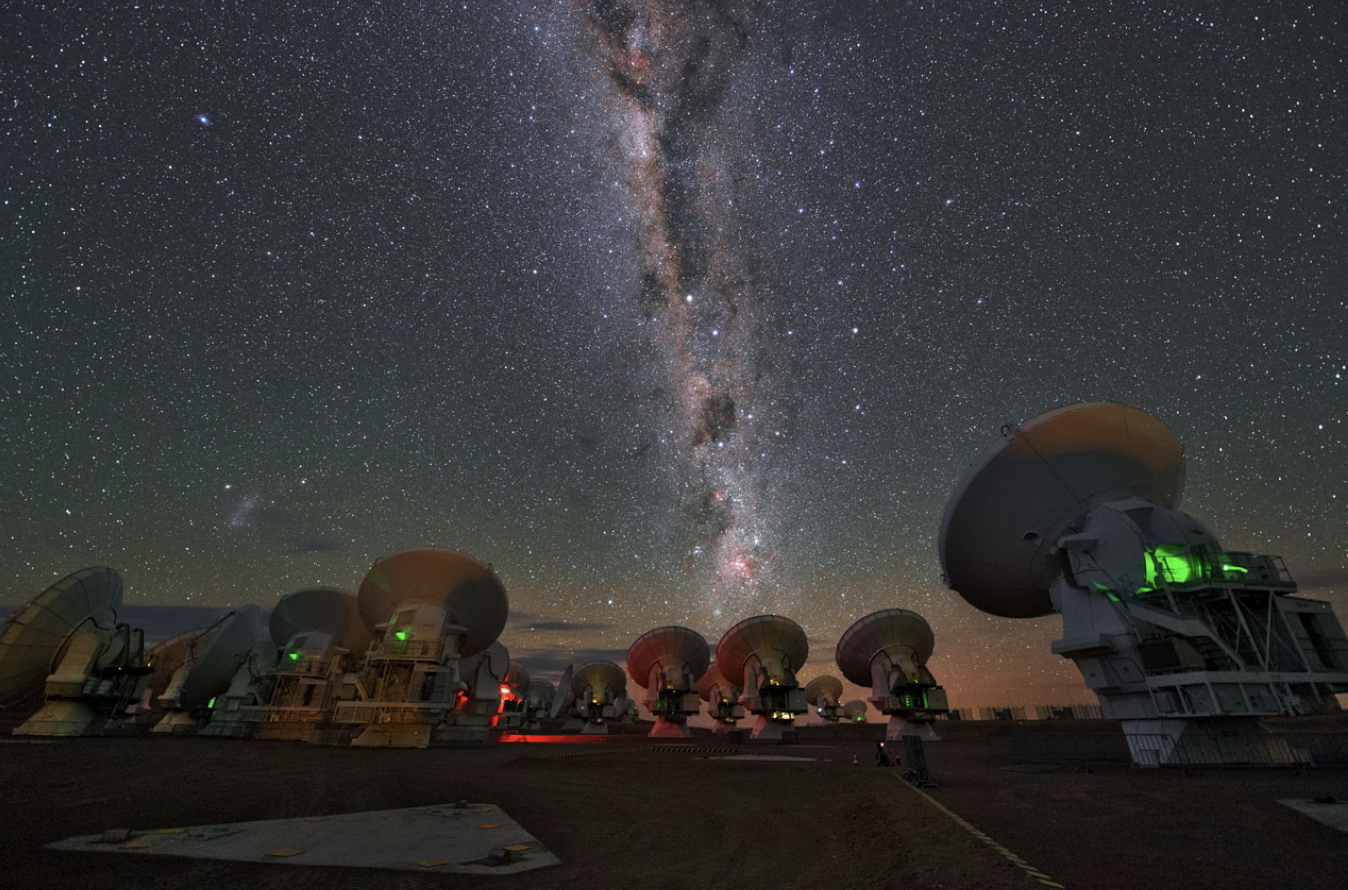
\includegraphics[scale=0.25]{media/radiotelescopes.png}\\
\column{0.5\textwidth}
\small Velkommen til andre forelesning av del 1D! Vi skal Vi skal gå rett over på spektrallinjer og undersøke hvordan disse oppstår, hvilken informasjon de bærer, hvordan vi kan modellere dem og analysere dem. Vi skal igjen innom minste kvadraters metode og $\chi^2$ i innleveringsoppgavene. Denne delen tilsvarer omkring en dobbelttime fysisk forelesning. \\{\bf Er du klar?}\\\vspace*{1cm}\hyperlink{intro2}{\pagebutton{Neste side}}
%\movie[autostart]{testmovie}{launch.gif}%bate2.mpg
\end{columns}
\end{frame}


\begin{frame}
\label{intro2}
\lastpagebutton{intro}
\vspace*{2cm}
La oss begynne med noen \href{https://nettskjema.no/a/155786}{spørsmål til ettertanke}. Vi skal jobbe videre med disse spørsmålene på neste side, så {\bf du trenger å ha tenkt gjennom og svart på spørsmålene før du går videre!}\\
\vspace*{1cm}
\href{https://nettskjema.no/a/155786}{\pagebutton{La meg kikke på spørsmålene en gang til slik at jeg er klar}}\\
\vspace*{1cm}
\hyperlink{blue_nytema1}{\pagebutton{\small Nå har jeg tenkt nøye gjennom spørsmålene og er klar til å fortsette}}
\end{frame}

\renewcommand{\headline}{\small Spektrallinjer}
{
\setbeamercolor{background canvas}{bg=blue}
\begin{frame}
\label{blue_nytema1}
\hyperlink{intro2}{\pagebutton{\small Forrige side}}
\nytemaside{bredde}
\hyperlink{linjeintro1}{\pagebutton{Sett igang med nytt og spennende tema!}}
\end{frame}
}


\begin{frame}
\label{linjeintro1}
\lastpagebutton{intro2}
Husker du Bohr atommodell? Den er illustert i \href{https://no.wikipedia.org/wiki/Bohrs_atommodell\#/media/Fil:Bohr_atom_animation_2.gif}{denne animasjonen på Wikipedia}. 
\begin{itemize}
\item Elektronene i atomene har kvantiserte energinivåer (representert som baner i animasjonen). Hvis en lyspartikkel (foton) med energi som tilsvarer nøyaktig forskjellen i to energinivåer passerer atomet, så kan elektronet absorpere dette fotonet, og hoppe et energinivå opp. 
\item Elektronene prøver å ha et lavest mulig energinivå slik at de etter kort tid faller ned igjen og sender dermed ut et foton som tilsvarer forskjellen i energi mellom energinivåene.
\end{itemize}
Du husker kanskje at energien til et foton er gitt ved
\[
E=h\nu=\frac{hc}{\lambda}
\]
???\\
Denne er så viktig at bør du huske den. Lys som har en bølgelengde $\lambda$ slik at energien $E$ tilsvarer overgangen mellom to energinivåer i et atom blir absorbert. Tilsvarende, når elektronet faller ned igjen, så sender det ut lys med bølgelengde $\lambda$ som da tilsvarer denne energien $E$.
\hyperlink{linjeintro2}{\pagebutton{Neste side}}
\end{frame}

\begin{frame}
\label{linjeintro2}
\begin{columns}
\column{0.5\textwidth}
\lastpagebuttoncr{linjeintro1}
Her ser vi dannelsen av en absorpsjonsline i atmosfæren til en stjerne (atmosfæren til stjerna, merket som 'Absorbing gas' er her skjematisk tegnet separat fra stjerna):
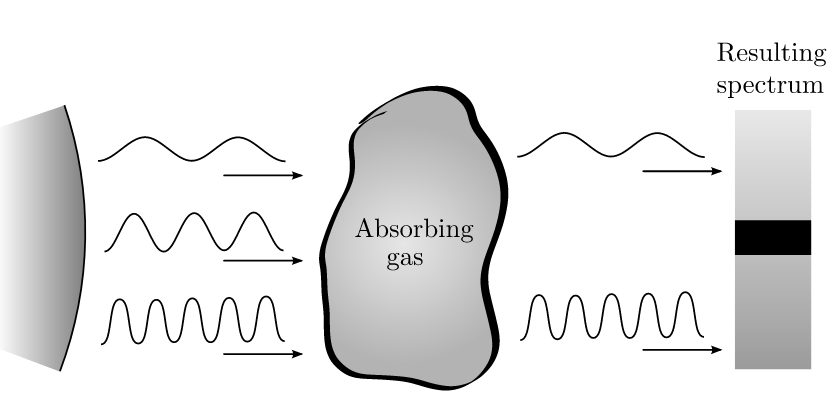
\includegraphics[scale=0.4]{media/absline.png}
\column{0.5\textwidth}
Gassen i atmosfæren inneholder atomer eller molekyler med energinivå som tilsvarer bølgelengden som vi ser blir absorbert. Dermed ser vi at disse bølgelengdene ikke kommer frem til observatøren med spektroskop på høyre side. Dermed blir det en mørk linje i spektret. \textcolor{red}{\bf Men vi lærte på forrige side at elektronene faller ned igjen og dermed sender ut fotonet med akkurat denne bølgelengden på nytt. Hvorfor blir det likevel en mørk linje i spektret?}
\end{columns}
\hyperlink{riktig_linjeintro3a}{\pagebutton{Jeg tror jeg vet hvorfor!}}\ \ \ \ \hyperlink{feil_linjeintro3b}{\pagebutton{Hæææ! Det var jo rart, hvordan kan det ha seg?}}
\end{frame}

{
\setbeamercolor{background canvas}{bg=black}
\begin{frame}
\label{feil_linjeintro3b}
\lastpagebutton{linjeintro2}
\textcolor{white}{{\bf Et lite hint:} Når elektronet sender ut fotonet igjen, blir det da alltid sendt mot observatøren? Hvor blir det sendt?}
\hyperlink{riktig_linjeintro3a}{\pagebutton{Neste side}}
\end{frame}
}

{
\setbeamercolor{background canvas}{bg=yellow}
\begin{frame}
\label{riktig_linjeintro3a}
\clastpagebutton{linjeintro2}
Årsaken er at elektronet ikke aner noe om hvor fotonet kom fra, det aner ikke engang at det ble løftet opp i et nytt energinivå pga. av et foton (et elektron aner strengt tatt ingenting, all forskning så langt peker på at elektroner ikke er bevisst...). Dermed blir dette fotonet sendt ut i en helt tilfeldig retning. Noen slike fotoner vil tilfeldigvis faktisk gå i retning av observatøren men langt mindre lys på denne bølgelengden vil komme frem, siden de aller fleste blir spredd i alle andre retninger.
\hyperlink{linjeintro4}{\pagebutton{Neste side}}
\end{frame}
}


\begin{frame}
\label{linjeintro4}
\lastpagebutton{riktig_linjeintro3a}
\begin{columns}
\column{0.5\textwidth}
Hva så med denne emisjonslinja da? Her ser vi det illustrert:
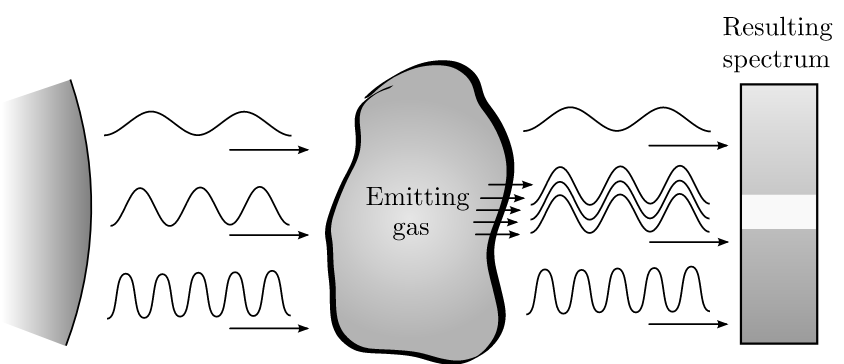
\includegraphics[scale=0.4]{media/emline.png}
Hvilken prosess gjør at vi får ekstra mange fotoner på en gitt bølgelengde?
\hyperlink{linjeintro4_b}{\choicebutton{Jeg har en aning om hvorfor}}\ \ \ \ \hyperlink{linjeintro4_c}{\choicebutton{Det vakke lett å se...}}\\
\column{0.5\textwidth}
\textcolor{white}{
{\bf Et hint:} Kan du tenke deg en annen prosess som gjør at elektronet hopper opp?\\
{Tjaaaa, kanskje det?}\\
Hvis gassen har høy temperatur, vil partiklene skumpe borti hverandre og overføre energi slik at elektronet kan hoppe opp. Men som før vil det falle ned igjen, og sende ut ekstra mange fotoner på akkurat bølgelgenden som tilsvarer denne energiforskjellen.
{Neste side}}
\end{columns}
\end{frame}

\begin{frame}
\label{linjeintro4_b}
\lastpagebutton{riktig_linjeintro3a}
\begin{columns}
\column{0.5\textwidth}
Hva så med denne emisjonslinja da? Her ser vi det illustrert:
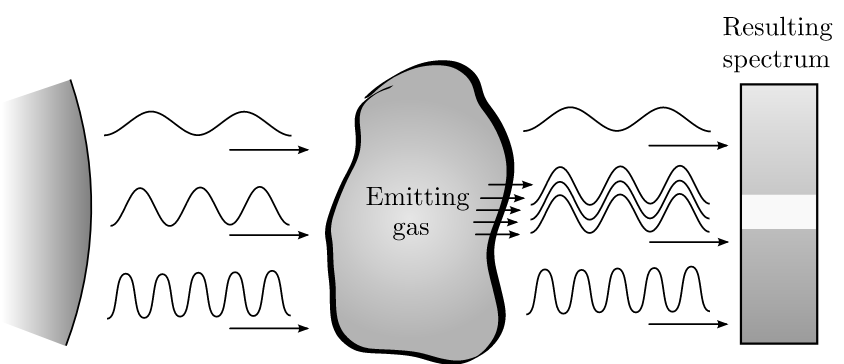
\includegraphics[scale=0.4]{media/emline.png}
Hvilken prosess gjør at vi får ekstra mange fotoner på en gitt bølgelengde?
{\choicebutton{Jeg har en aning om hvorfor}}\ \ \ \ {\choicebutton{Det vakke lett å se...}}\\
\column{0.5\textwidth}
{\bf Et hint:} Kan du tenke deg en annen prosess som gjør at elektronet hopper opp?\\
\hyperlink{linjeintro4_c}{\choicebutton{Tjaaaa, kanskje det?}}\\
\textcolor{white}{
Hvis gassen har høy temperatur, vil partiklene skumpe borti hverandre og overføre energi slik at elektronet kan hoppe opp. Men som før vil det falle ned igjen, og sende ut ekstra mange fotoner på akkurat bølgelgenden som tilsvarer denne energiforskjellen.
{Neste side}}
\end{columns}
\end{frame}

\begin{frame}
\label{linjeintro4_c}
\lastpagebutton{riktig_linjeintro3a}
\begin{columns}
\column{0.5\textwidth}
Hva så med denne emisjonslinja da? Her ser vi det illustrert:
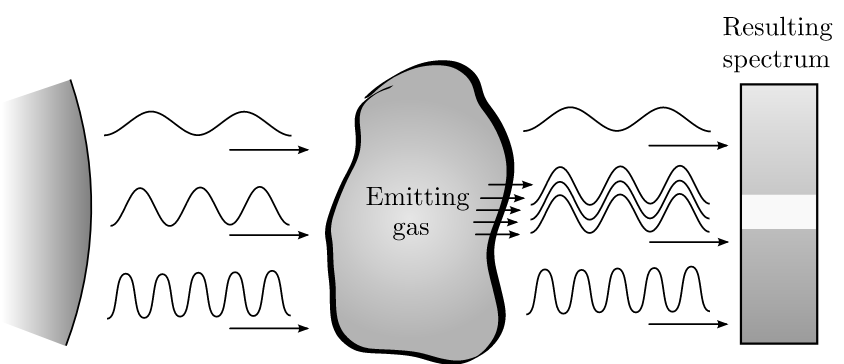
\includegraphics[scale=0.4]{media/emline.png}
Hvilken prosess gjør at vi får ekstra mange fotoner på en gitt bølgelengde?
{\choicebutton{Jeg har en aning om hvorfor}}\ \ \ \ \ {\choicebutton{Det vakke lett å se...}}\\
\column{0.5\textwidth}
{\bf Et hint:} Kan du tenke deg en annen prosess som gjør at elektronet hopper opp?\\
{\choicebutton{Tjaaaa, kanskje det?}}\\
Hvis gassen har høy temperatur, vil partiklene skumpe borti hverandre og overføre energi slik at elektronet kan hoppe opp. Men som før vil det falle ned igjen, og sende ut ekstra mange fotoner på akkurat bølgelgenden som tilsvarer denne energiforskjellen.
\hyperlink{blue_nytema2}{\pagebutton{Neste side}}
\end{columns}
\end{frame}

\renewcommand{\headline}{\small Bredden til spektrallinjer}
{
\setbeamercolor{background canvas}{bg=blue}
\begin{frame}
\label{blue_nytema2}
\hyperlink{linjeintro4}{\pagebutton{\small Forrige side}}
\nytemaside{form}
\hyperlink{linjeintro5}{\pagebutton{Kom igjen, la oss se hva som gir linjene bredde!}}
\end{frame}
}


\begin{frame}
\label{linjeintro5}
\begin{columns}
\column{0.5\textwidth}
\dlastpagebutton{linjeintro4}\label{bredde}
Tilbake til spørsmålet fra skjemaet: vi bruker illustrasjonen av absorpsjonsline. {\bf Anta at atmosfæren (den absorberende gassen) er i ro i forhold til stjerna og observatøren} (spektrografen til høyre):
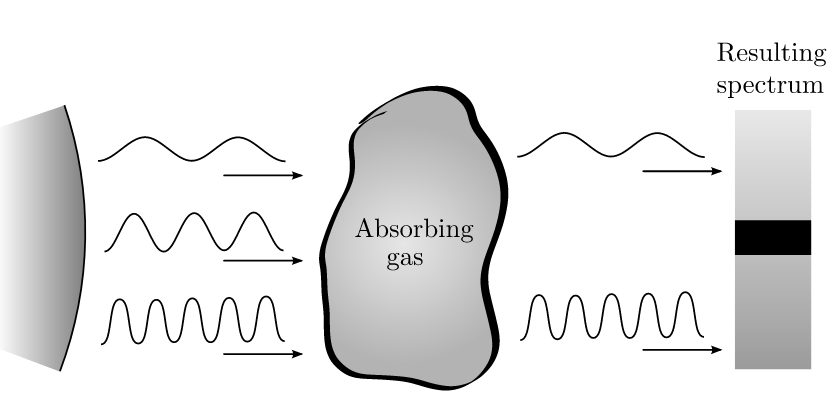
\includegraphics[scale=0.4]{media/absline.png}
{\bf Vi antar at gasspartiklene kun absorberer på bølgelengde $\lambda_0$.} Vi vet at gasspartiklene har tilfeldige hastigheter i tilfeldige retninger fra Maxwell-Boltzmann-fordelingen.
\column{0.5\textwidth}
Et atom i den absorberende gassen som har hastighet mot stjerna absorberer et foton. Hvordan vil en obsevatør på dette atomet oppleve stjerna?
\hyperlink{linjeintro5_a}{\pagebutton{\small Stjerna står i ro}}\ \ \ \ \hyperlink{linjeintro6}{\pagebutton{\small Stjerna beveger seg mot atomet}}\ \ \ \ \hyperlink{linjeintro5_a}{\pagebutton{\small Stjerna beveger seg fra atomet}}\\
\textcolor{white}{Et lite hint for å hjelpe til: hvis du kjører bil mot en bygning, i ditt referansesystem, beveger bygningen seg mot deg, fra deg, eller er den i ro?
Ahhh, nå ser jeg det!}
\end{columns}
\end{frame}



\begin{frame}
\label{linjeintro5_a}
\begin{columns}
\column{0.5\textwidth}
\dlastpagebutton{linjeintro4}\label{bredde}
Tilbake til spørsmålet fra skjemaet: vi bruker illustrasjonen av absorpsjonsline. {\bf Anta at atmosfæren (den absorberende gassen) er i ro i forhold til stjerna og observatøren} (spektrografen til høyre):
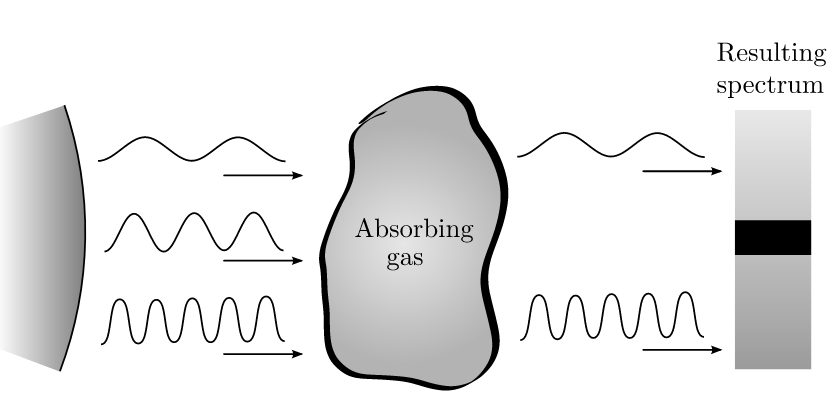
\includegraphics[scale=0.4]{media/absline.png}
{\bf Vi antar at gasspartiklene kun absorberer på bølgelengde $\lambda_0$.} Vi vet at gasspartiklene har tilfeldige hastigheter i tilfeldige retninger fra Maxwell-Boltzmann-fordelingen.
\column{0.5\textwidth}
Et atom i den absorberende gassen som har hastighet mot stjerna absorberer et foton. Hvordan vil en obsevatør på dette atomet oppleve stjerna?
{\pagebutton{\small Stjerna står i ro}}\ \ \ \ {\pagebutton{\small Stjerna beveger seg mot atomet}}\ \ \ \ {\pagebutton{\small Stjerna beveger seg fra atomet}}\\
Et lite hint for å hjelpe til: hvis du kjører bil mot en bygning, i ditt referansesystem, beveger bygningen seg mot deg, fra deg, eller er den i ro?
\hyperlink{linjeintro6}{\pagebutton{Ahhh, nå ser jeg det!}}
\end{columns}
\end{frame}

\begin{frame}
\label{linjeintro6}
\begin{columns}
\column{0.5\textwidth}
\addtocounter{pageno}{1}
\dlastpagebutton{linjeintro5}
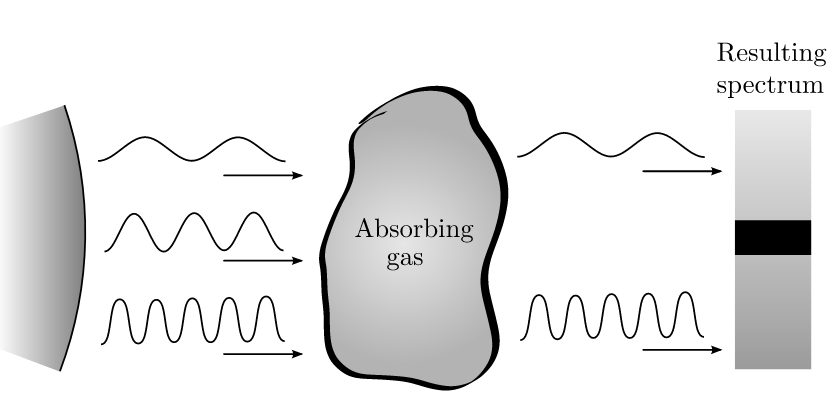
\includegraphics[scale=0.4]{media/absline.png}
Korrekt, for atomet som går i retning mot stjerna vil det virke som at stjerna beveger seg mot atomet. Vil det ha en innvirkning på bølgelengden som elektronet i atomet absorberer? Tenk deg et foton sendt ut med bølgelengde $\lambda_0$ fra stjerna. Hvilken bølgelengde har dette fotonet i atomet sitt referansesystem?\\
\vspace*{0.5cm}
\hyperlink{linjeintro6_b}{\choicebutton{\small fortsatt $\lambda_0$}}\ \ \ \ \hyperlink{linjeintro6_b}{\choicebutton{\small større enn $\lambda_0$}}\ \ \ \ \hyperlink{riktig_linjeintro7}{\choicebutton{\small mindre enn $\lambda_0$}}
\column{0.5\textwidth}
\textcolor{white}{Det ble feil!
Husker du Doppler-effekten? Hva skjer hvis en lyskilde beveger seg {\bf mot} deg?
Ahhh, nå ser jeg det!}
\end{columns}
\end{frame}

\begin{frame}
\label{linjeintro6_b}
\begin{columns}
\column{0.5\textwidth}
\addtocounter{pageno}{1}
\dlastpagebutton{linjeintro5}
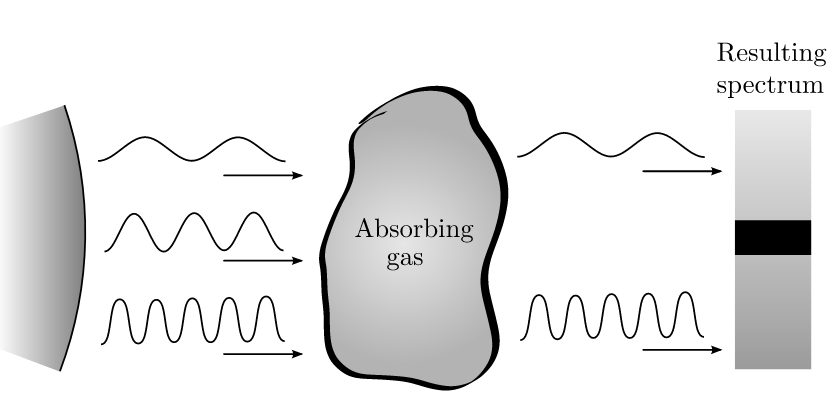
\includegraphics[scale=0.4]{media/absline.png}
Korrekt, for atomet som går i retning mot stjerna vil det virke som at stjerna beveger seg mot atomet. Vil det ha en innvirkning på bølgelengden som elektronet i atomet absorberer? Tenk deg et foton sendt ut med bølgelengde $\lambda_0$ fra stjerna. Hvilken bølgelengde har dette fotonet i atomet sitt referansesystem?\\
\vspace*{0.5cm}
\hyperlink{linjeintro6_b}{\choicebutton{\small fortsatt $\lambda_0$}}\ \ \ \ \hyperlink{linjeintro6_b}{\choicebutton{\small større enn $\lambda_0$}}\ \ \ \ \hyperlink{riktig_linjeintro7}{\choicebutton{\small mindre enn $\lambda_0$}}
\column{0.5\textwidth}
\textcolor{red}{Det ble feil!}
Husker du Doppler-effekten? Hva skjer hvis en lyskilde beveger seg {\bf mot} deg?
\hyperlink{riktig_linjeintro7}{\pagebutton{Ahhh, nå ser jeg det!}}
\end{columns}
\end{frame}



{
\setbeamercolor{background canvas}{bg=yellow}
\begin{frame}
\label{riktig_linjeintro7}
\begin{columns}
\column{0.5\textwidth}
\addtocounter{pageno}{2}
\dlastpagebuttoncr{linjeintro6}
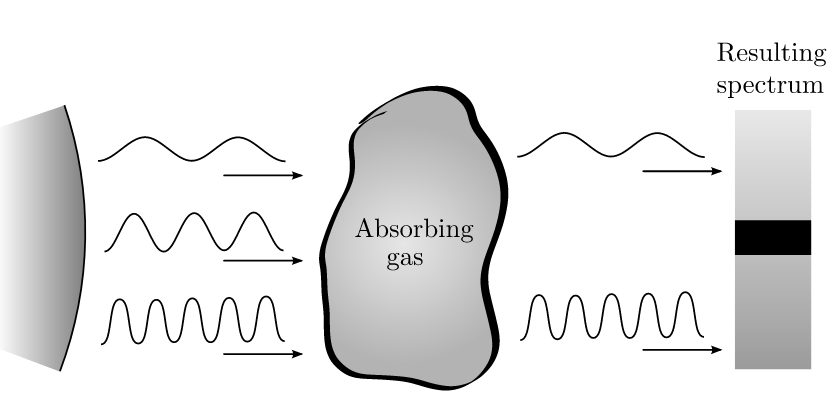
\includegraphics[scale=0.4]{media/absline.png}
Korrekt: Når atomet beveger seg mot stjerna, så vil, i atomets referansesystem, stjerna bevege seg mot atomet. Husk {\bf Doppler effekten}: Hvis en lyskilde beveger seg mot deg, vil du observere en {\bf kortere} bølgelengde! Lysbølgene som atomet observerer til å ha en bølgelengde $\lambda_0$ har dermed egentlig en {\bf lengre} bølgelengde sett fra stjerna (observatørens) referansesystem. 
\column{0.5\textwidth}
Atomet absorberer dermed en bølgelengde som er {\bf lengre} enn $\lambda_0$ sett fra observatøren! Ser du dermed også at de atomene som beveger seg med hastighet bort fra stjerna vil absorbere en bølgelengde som er kortere enn $\lambda_0$? Og de atomene som står omtrent i ro i forhold til stjerna vil absorbere omtrent på bølgelengden $\lambda_0$? På grunn av gasspartiklenes tilfeldig bevegelse inne i gassen, så vil vi, selv om gassen som helhelt står i ro i forhold til stjerna,{\bf  få absorpsjon både på $\lambda_0$, men også på andre bølgelengder i nærheten av $\lambda_0$.}. Dette som et resultat av Dopplereffekten fra atomenes tilfeldige bevegelser inne i gassen.
\hyperlink{linjeintro8}{\pagebutton{Neste side}}
\end{columns}
\end{frame}
}

\begin{frame}
\label{linjeintro8}
\lastpagebutton{riktig_linjeintro7}
Vi får dermed en bredde på linja, og {\bf ikke} en syltynn spektrallinje på nøyaktig bølgelengden $\lambda_0$:
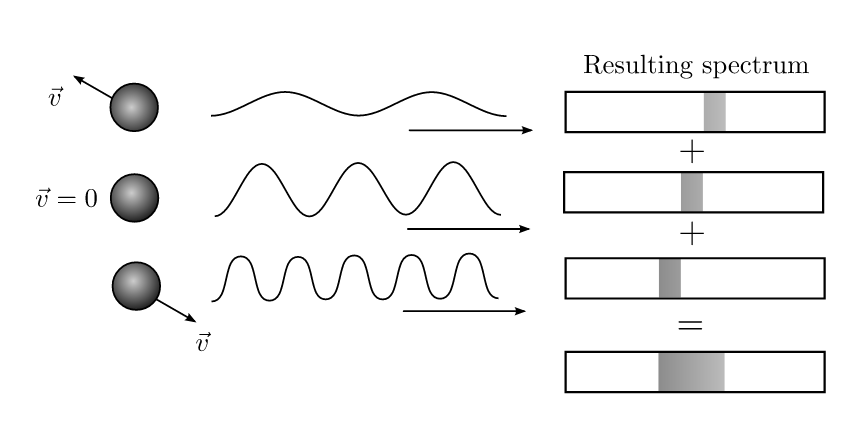
\includegraphics[scale=0.6]{media/linewidth.png}\\
\textcolor{red}{Men hvor bred blir linja og hva avgjør det? Og hva blir formen på linja?}
{\bf Kan du allerede tenke deg hvilken egenskap ved gassen som avgjør hvor bred linja blir??}
\hyperlink{blue_nytema3}{\pagebutton{Neste side}}
\end{frame}

\renewcommand{\headline}{\small Formen til spektrallinjer}
{
\setbeamercolor{background canvas}{bg=blue}
\begin{frame}
\label{blue_nytema3}
\hyperlink{linjeintro8}{\pagebutton{\small Forrige side}}
\nytemaside{obs}
\hyperlink{linjeintro9}{\pagebutton{La oss modellere formen til spektrallinjene!}}
\textcolor{yellow}{og ved neste tema tror jeg du trenger en skikkelig pause!}
\end{frame}
}


\begin{frame}
\label{linjeintro9}
\lastpagebutton{linjeintro8}\label{form}
Før vi svarer på spørsmålet, la oss undersøke litt. Hvis vi setter \textcolor{red}{en x-akse som går fra observatøren, gjennom gassen og mot stjerna}, er du da enig i at hastighetskomponenten i gassen som avgjør Doppler-effekten er x-komponenten av partikkelhastigheten? {\bf Altså $v_x$ til partiklene avgjør hvilken bølgelengde $\lambda$ som blir absorbert?}
\hyperlink{linjeintro9_b}{\choicebutton{Ja,helt enig!}}\ \ \ \ \hyperlink{linjeintro9_b}{\choicebutton{Nja, tror det...}}
\textcolor{white}{
{\bf Hvis du er usikker, kontakt foreleser nå før du går videre!}\\
Hastighetskomponenten $v_x$ avgjør i hvilken retning og hvor fort stjerna beveger seg i forhold til gasspartikkelen, og dermed hvilken Dopplereffekt vi får på den innkomne bølgelengden og dermed hvilken bølgelengde som blir absorbert. Tenk deg {\bf at en gasspartikkel har negativ hastighet $-v_x$ i forhold til stjerna.} Hvilken bølgelengde $\lambda$ blir absorbert av denne gasspartikkelen?  {\bf Pass på retningen på aksen og fortegn her!}
$\lambda_0$\ \ \ \ $\lambda_0v_x$\ \ \ \ $\frac{\lambda_0}{v_x}$\ \ \ \ $\lambda_0\frac{v_x}{c}$\ \ \ \ $\lambda_0+\lambda_0\frac{v_x}{c}$\ \ \ \ $\lambda_0-\lambda_0\frac{v_x}{c}$\ \ \ \ $\lambda_0+\frac{\lambda_0}{c}$\ \ \ \ $\lambda_0-\frac{\lambda_0}{c}$\ \ \ \ $+\frac{\lambda_0}{c}$\ \ \ \ $-\frac{\lambda_0}{c}$\ \ \ \ $-\frac{v_x}{c}$
}
\end{frame}

\begin{frame}
\label{linjeintro9_b}
\lastpagebutton{linjeintro8}\label{form}
Før vi svarer på spørsmålet, la oss undersøke litt. Hvis vi setter \textcolor{red}{en x-akse som går fra observatøren, gjennom gassen og mot stjerna}, er du da enig i at hastighetskomponenten i gassen som avgjør Doppler-effekten er x-komponenten av partikkelhastigheten? {\bf Altså $v_x$ til partiklene avgjør hvilken bølgelengde $\lambda$ som blir absorbert?}
\hyperlink{linjeintro9_b}{\choicebutton{Ja,helt enig!}}\ \ \ \ \hyperlink{linjeintro9_b}{\choicebutton{Nja, tror det...}}
{\bf Hvis du er usikker, kontakt foreleser nå før du går videre!}\\
Hastighetskomponenten $v_x$ avgjør i hvilken retning og hvor fort stjerna beveger seg i forhold til gasspartikkelen, og dermed hvilken Dopplereffekt vi får på den innkomne bølgelengden og dermed hvilken bølgelengde som blir absorbert. Tenk deg {\bf at en gasspartikkel har negativ hastighet $-v_x$ i forhold til stjerna.} Hvilken bølgelengde $\lambda$ blir absorbert av denne gasspartikkelen?  {\bf Pass på retningen på aksen og fortegn her!}
\hyperlink{feillambda}{\choicebutton{$\lambda_0$}}\ \ \ \ \hyperlink{feillambda}{\choicebutton{$\lambda_0v_x$}}\ \ \ \ \hyperlink{feillambda}{\choicebutton{$\frac{\lambda_0}{v_x}$}}\ \ \ \ \hyperlink{feillambda}{\choicebutton{$\lambda_0\frac{v_x}{c}$}}\ \ \ \ \hyperlink{feillambda}{\choicebutton{$\lambda_0+\lambda_0\frac{v_x}{c}$}}\ \ \ \ \hyperlink{riktiglambda}{\choicebutton{$\lambda_0-\lambda_0\frac{v_x}{c}$}}\ \ \ \ \hyperlink{feillambda}{\choicebutton{$\lambda_0+\frac{\lambda_0}{c}$}}\ \ \ \ \hyperlink{feillambda}{\choicebutton{$\lambda_0-\frac{\lambda_0}{c}$}}\ \ \ \ \hyperlink{feillambda}{\choicebutton{$+\frac{\lambda_0}{c}$}}\ \ \ \ \hyperlink{feillambda}{\choicebutton{$-\frac{\lambda_0}{c}$}}\ \ \ \ \hyperlink{feillambda}{\choicebutton{$-\frac{v_x}{c}$}}
\end{frame}




{
\setbeamercolor{background canvas}{bg=black}
\begin{frame}
\label{feillambda}
\dlastpagebutton{linjeintro9_b}
\textcolor{white}{Det ble galt! Husker du Dopplerformelen? Den {\bf må} du kunne i dette kurset. Gå tilbake til del 1C og forsikre deg om at du virkelig kan dette med Doppler effekten! Du må også ha helt klart for deg når bølgelgenden blir kortere og når den blir lengre! Du fikk oppgitt at hastigheten er negativ, hvilken retning går den da i forhold til stjerna? Blir bølgelengden lengre eller kortere? Gå tilbake og prøv igjen! Hvis du ikke får det til, {\bf kontakt foreleser nå!!!!}}
\end{frame}
}

{
\setbeamercolor{background canvas}{bg=yellow}
\begin{frame}
\label{riktiglambda}
\clastpagebutton{linjeintro9}
Flott! Du har forstått det!Hvis du likevel er usikker, {\bf kontakt foreleser nå!!!!}
Spørsmålet nå blir da hvor mange gasspartikler har en gitt hastighet $v_x$ og som dermed gir en gitt Dopplereffekt $\frac{v_x}{c}$?? Vel, vi vet vel allerede svaret: {\bf Maxwell-Boltzmannfordelingen for hastighetskomponenter!} Husker du hvordan den ser ut?

\hyperlink{riktiglambda_b}{\choicebutton{\small Hvordan kunne jeg glemme det??}}\ \ \ \ \hyperlink{riktiglambda_b}{\choicebutton{\small Ikke med en gang, men nå gikk jeg tilbake til 1A og repeterte!}}\\
\textcolor{yellow}{
Stemmer, det er en Gaussisk fordeling med gjennomsnitt 0 og standardavvik på... husker du hvor stort standardavviket $\sigma$ var?
{\small Of course! Jeg har fotografisk minne!}\ \ \ \ \small Ikke med en gang, men nå gikk jeg tilbake til 1A og repeterte!\\
Stemmer, jammen var det
\[
\sigma=\sqrt{\frac{kT}{m}}
\]
Neste side}
\end{frame}
}


{
\setbeamercolor{background canvas}{bg=yellow}
\begin{frame}
\label{riktiglambda_b}
\clastpagebutton{linjeintro9}
Flott! Du har forstått det!Hvis du likevel er usikker, {\bf kontakt foreleser nå!!!!}
Spørsmålet nå blir da hvor mange gasspartikler har en gitt hastighet $v_x$ og som dermed gir en gitt Dopplereffekt $\frac{v_x}{c}$?? Vel, vi vet vel allerede svaret: {\bf Maxwell-Boltzmannfordelingen for hastighetskomponenter!} Husker du hvordan den ser ut?

{\choicebutton{\small Hvordan kunne jeg glemme det??}}\ \ \ \ {\choicebutton{\small Ikke med en gang, men nå gikk jeg tilbake til 1A og repeterte!}}\\
Stemmer, det er en Gaussisk fordeling med gjennomsnitt 0 og standardavvik på... husker du hvor stort standardavviket $\sigma$ var?
\hyperlink{riktiglambda_c}{\choicebutton{\small Of course! Jeg har fotografisk minne!}}\ \ \ \ \hyperlink{riktiglambda_c}{\choicebutton{\small Ikke med en gang, men nå gikk jeg tilbake til 1A og repeterte!}}\\
\textcolor{yellow}{
Stemmer, jammen var det
\[
\sigma=\sqrt{\frac{kT}{m}}
\]
Neste side}
\end{frame}
}


{
\setbeamercolor{background canvas}{bg=yellow}
\begin{frame}
\label{riktiglambda_c}
\clastpagebutton{linjeintro9}
Flott! Du har forstått det!Hvis du likevel er usikker, {\bf kontakt foreleser nå!!!!}
Spørsmålet nå blir da hvor mange gasspartikler har en gitt hastighet $v_x$ og som dermed gir en gitt Dopplereffekt $\frac{v_x}{c}$?? Vel, vi vet vel allerede svaret: {\bf Maxwell-Boltzmannfordelingen for hastighetskomponenter!} Husker du hvordan den ser ut?

{\choicebutton{\small Hvordan kunne jeg glemme det??}}\ \ \ \ {\choicebutton{\small Ikke med en gang, men nå gikk jeg tilbake til 1A og repeterte!}}\\
Stemmer, det er en Gaussisk fordeling med gjennomsnitt 0 og standardavvik på... husker du hvor stort standardavviket $\sigma$ var?
{\choicebutton{\small Of course! Jeg har fotografisk minne!}}\ \ \ \ {\choicebutton{\small Ikke med en gang, men nå gikk jeg tilbake til 1A og repeterte!}}\\
Stemmer, jammen var det
\[
\sigma=\sqrt{\frac{kT}{m}}
\]
\hyperlink{linjeintro10}{\pagebutton{Neste side}}
\end{frame}
}









\begin{frame}
\label{linjeintro10}
\lastpagebutton{riktiglambda}
Hvilken bølgelgende tror du da som det blir absorbert mest av? Hvor får vi sterkest absorpsjon i spektret?\\
\hyperlink{riktiglambda2}{\choicebutton{$\lambda_0$}}\ \ \ \ \hyperlink{feillambda2}{\choicebutton{$\lambda_0v_x$}}\ \ \ \ \hyperlink{feillambda2}{\choicebutton{$\frac{\lambda_0}{v_x}$}}\ \ \ \ \hyperlink{feillambda2}{\choicebutton{$\frac{v_x}{c}$}}\ \ \ \ \hyperlink{feillambda2}{\choicebutton{$\lambda_0+\frac{v_x}{c}$}}\ \ \ \ \hyperlink{feillambda2}{\choicebutton{$\lambda_0-\frac{v_x}{c}$}}\ \ \ \ \hyperlink{feillambda2}{\choicebutton{$\lambda_0+\frac{\lambda_0}{c}$}}\ \ \ \ \hyperlink{feillambda2}{\choicebutton{$\lambda_0-\frac{\lambda_0}{c}$}}\ \ \ \ \hyperlink{feillambda2}{\choicebutton{$+\frac{\lambda_0}{c}$}}\ \ \ \ \hyperlink{feillambda2}{\choicebutton{$-\frac{\lambda_0}{c}$}}\ \ \ \ \hyperlink{feillambda2}{\choicebutton{$-\frac{v_x}{c}$}}
\end{frame}


{
\setbeamercolor{background canvas}{bg=black}
\begin{frame}
\label{feillambda2}
\lastpagebutton{linjeintro10}
\textcolor{white}{Det ble ikke helt riktig! Kan du tegne Maxwell-Boltzmann-fordelingen for $v_x$? Hvilken hastighet $v_x$ har de fleste partiklene i gassen? Hvilken Dopplereffekt gir denne bølgelengden? Hva blir dermed bølgelengden som får sterkest absorpsjon? Gå tilbake og prøv igjen!}
\end{frame}
}

{
\setbeamercolor{background canvas}{bg=yellow}
\begin{frame}
\label{riktiglambda2}
\clastpagebutton{linjeintro10}
Det er helt riktig! Maxwell-Boltzmann-fordelingen for $v_x$ så slik ut:
\centerline{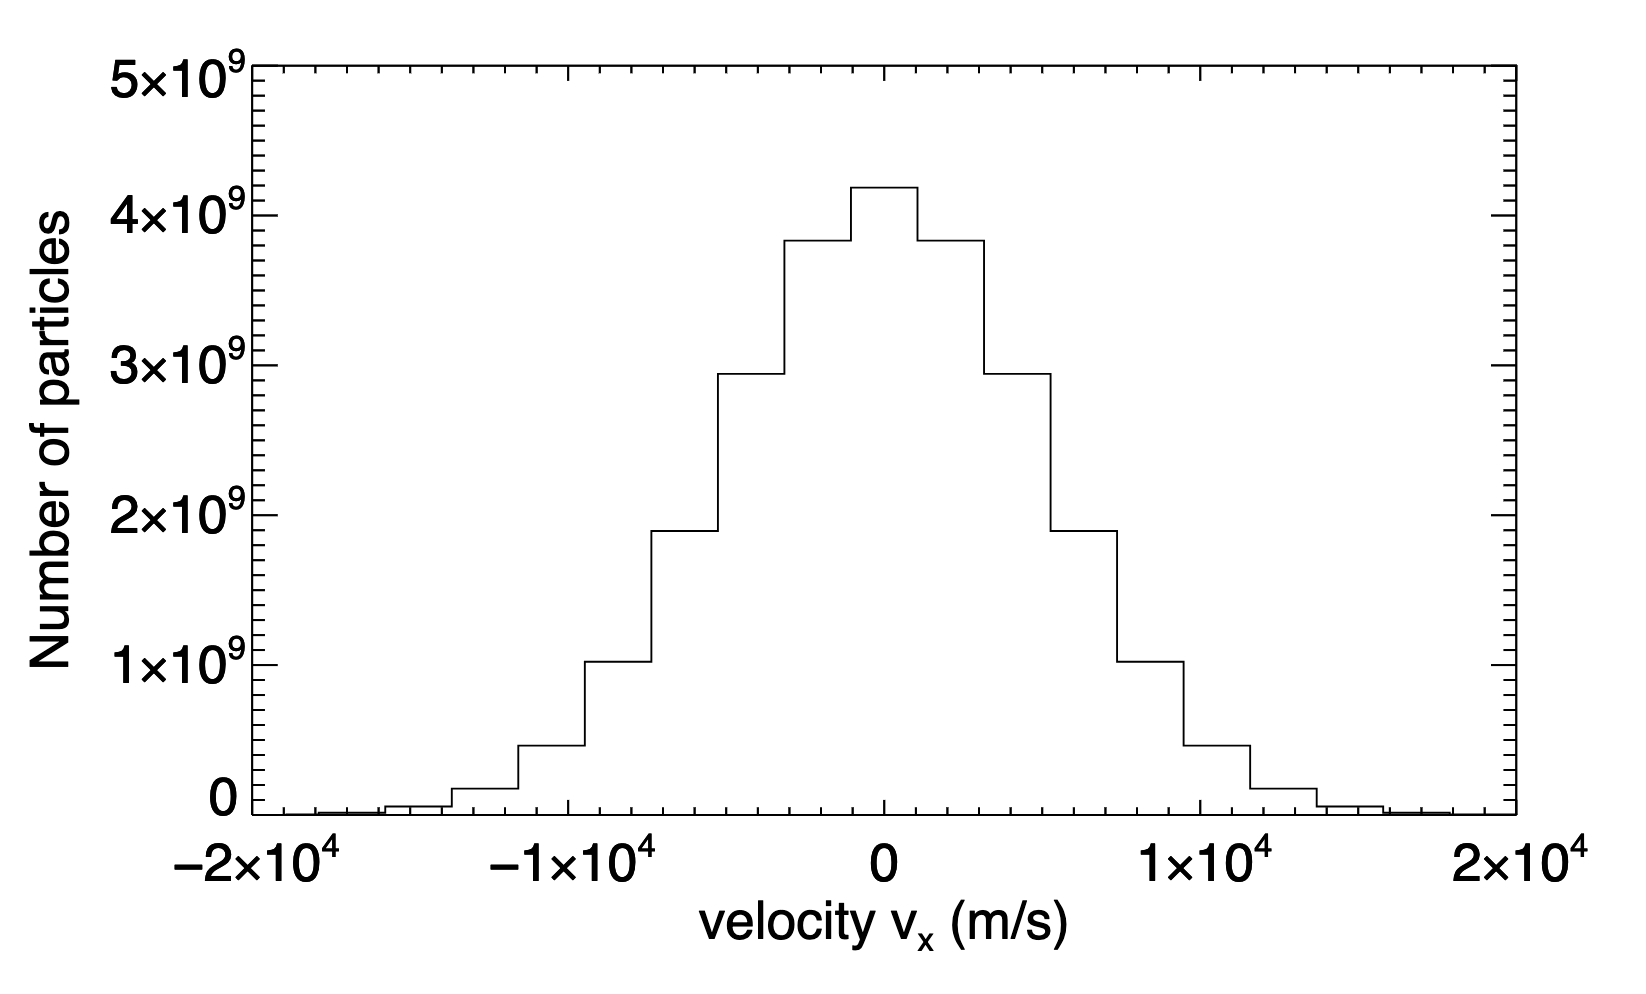
\includegraphics[scale=0.25]{media/vx_histogram.png}}
Ser du at de aller fleste partiklene har omkring 0 hastighet i x-retning? Dermed får du ingen Dopplereffekt fra de fleste partiklene. Dermed forblir absorpsjonen på bølgelgenden omkring $\lambda_0$ for det meste av strålingen.
\hyperlink{linjeintro11}{\pagebutton{Neste side}}
\end{frame}
}

\begin{frame}
\label{linjeintro11}
\lastpagebutton{riktiglambda2}
{\small Her ser vi hvordan partiklene med forskjellige hastigheter bidrar til absorpsjonslina:}
\centerline{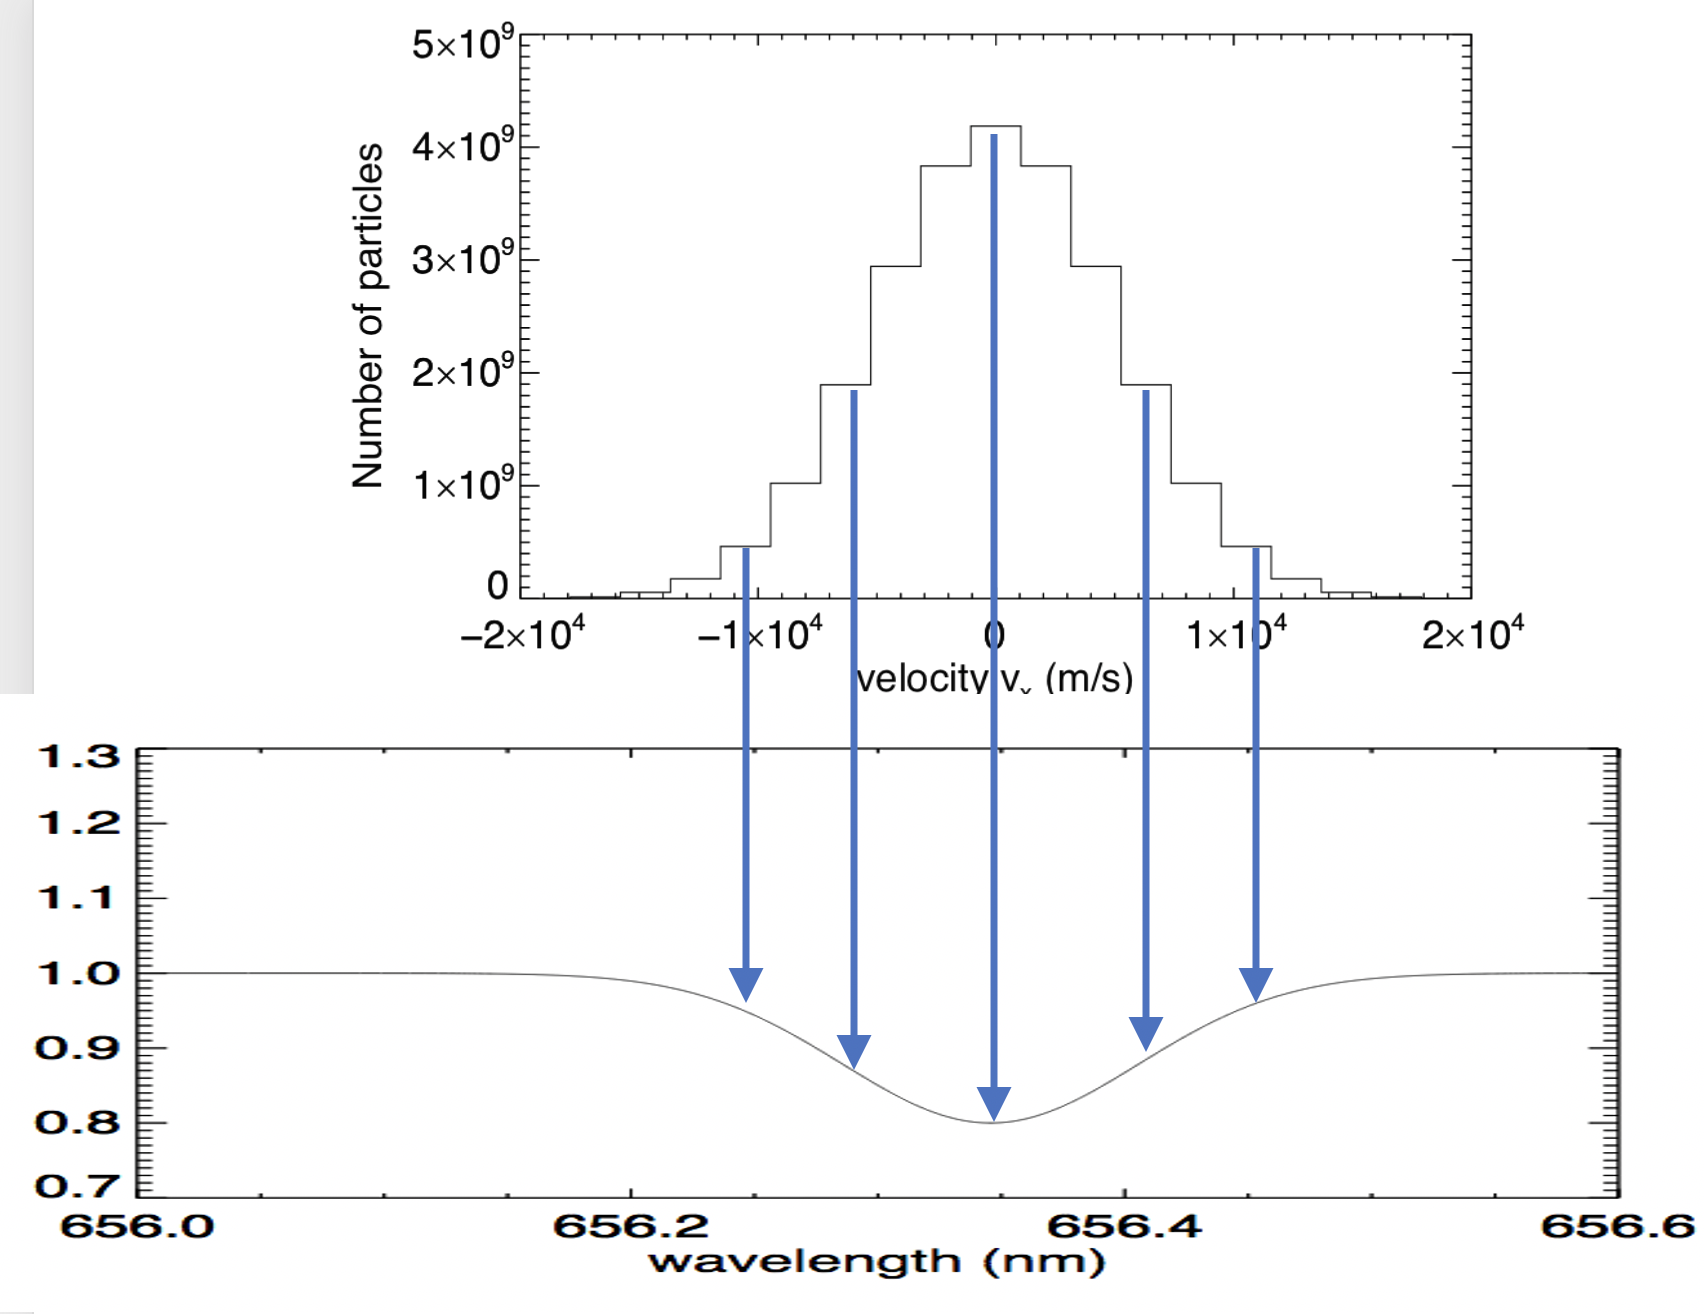
\includegraphics[scale=0.2]{media/linegen.png}}
{\small
Øverst har vi hastighetsfordelingen for $v_x$, nederst har vi fluksen $F(\lambda)$ som funksjon av bølgelengden. Vi har altså flest partikler med $v_x$ omkring 0 som gir bidrag til absorpsjonen ved $\lambda_0$. Siden det er flest partikler som absorberer på denne bølgelengden blir det også størst absorpsjon der. For hastigheter $|v_x|>0$ ser vi at vi har færre partikler, dermed også svakere absorpsjon. Helt på enden av fordelingen hvor det er nesten 0 partikler får vi da heller nesten ingen absorpsjon.
}
\hyperlink{linjeintro12}{\pagebutton{Neste side}}
\end{frame}


\begin{frame}
\label{linjeintro12}
\lastpagebutton{linjeintro11}
\centerline{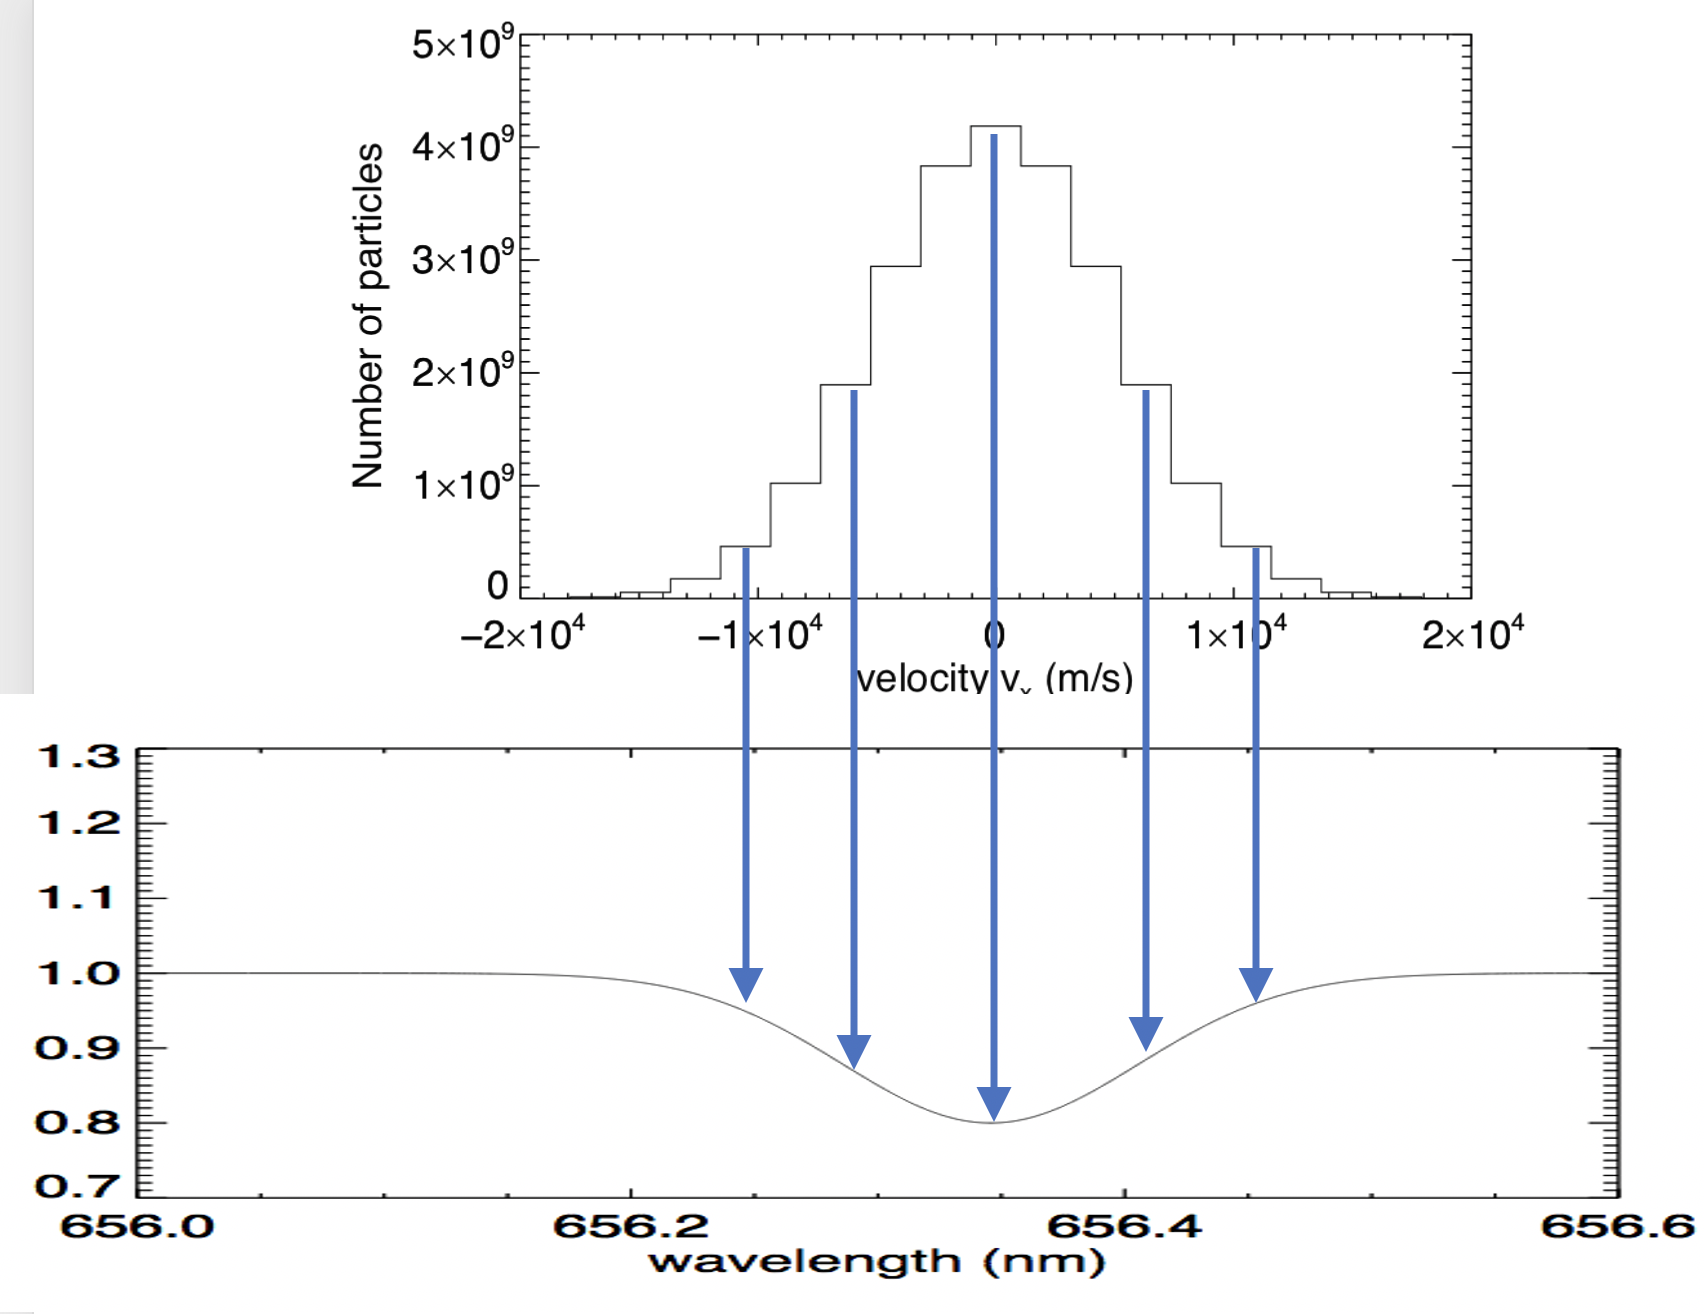
\includegraphics[scale=0.2]{media/linegen.png}}
{\small
Ser du at hvor sterk absorpsjon du får er proporsjonalt med antall partikler som har den gitte hastigheten? Hvis dobbelt så mange partikler har en gitt hastighet så vil også dobbelt så mange fotoner bli absorbert på den tilsvarende bølgelengden. Kan du dermed se hvordan formen på spektrallinja vil være? Hva slags form vil $F(\lambda)$ ha nær spektrallinja? Tenk deg om to ganger før du går videre.
}
\hyperlink{linjeintro13}{\pagebutton{Neste side}}
\end{frame}

\begin{frame}
\label{linjeintro13}
\lastpagebutton{linjeintro12}
\centerline{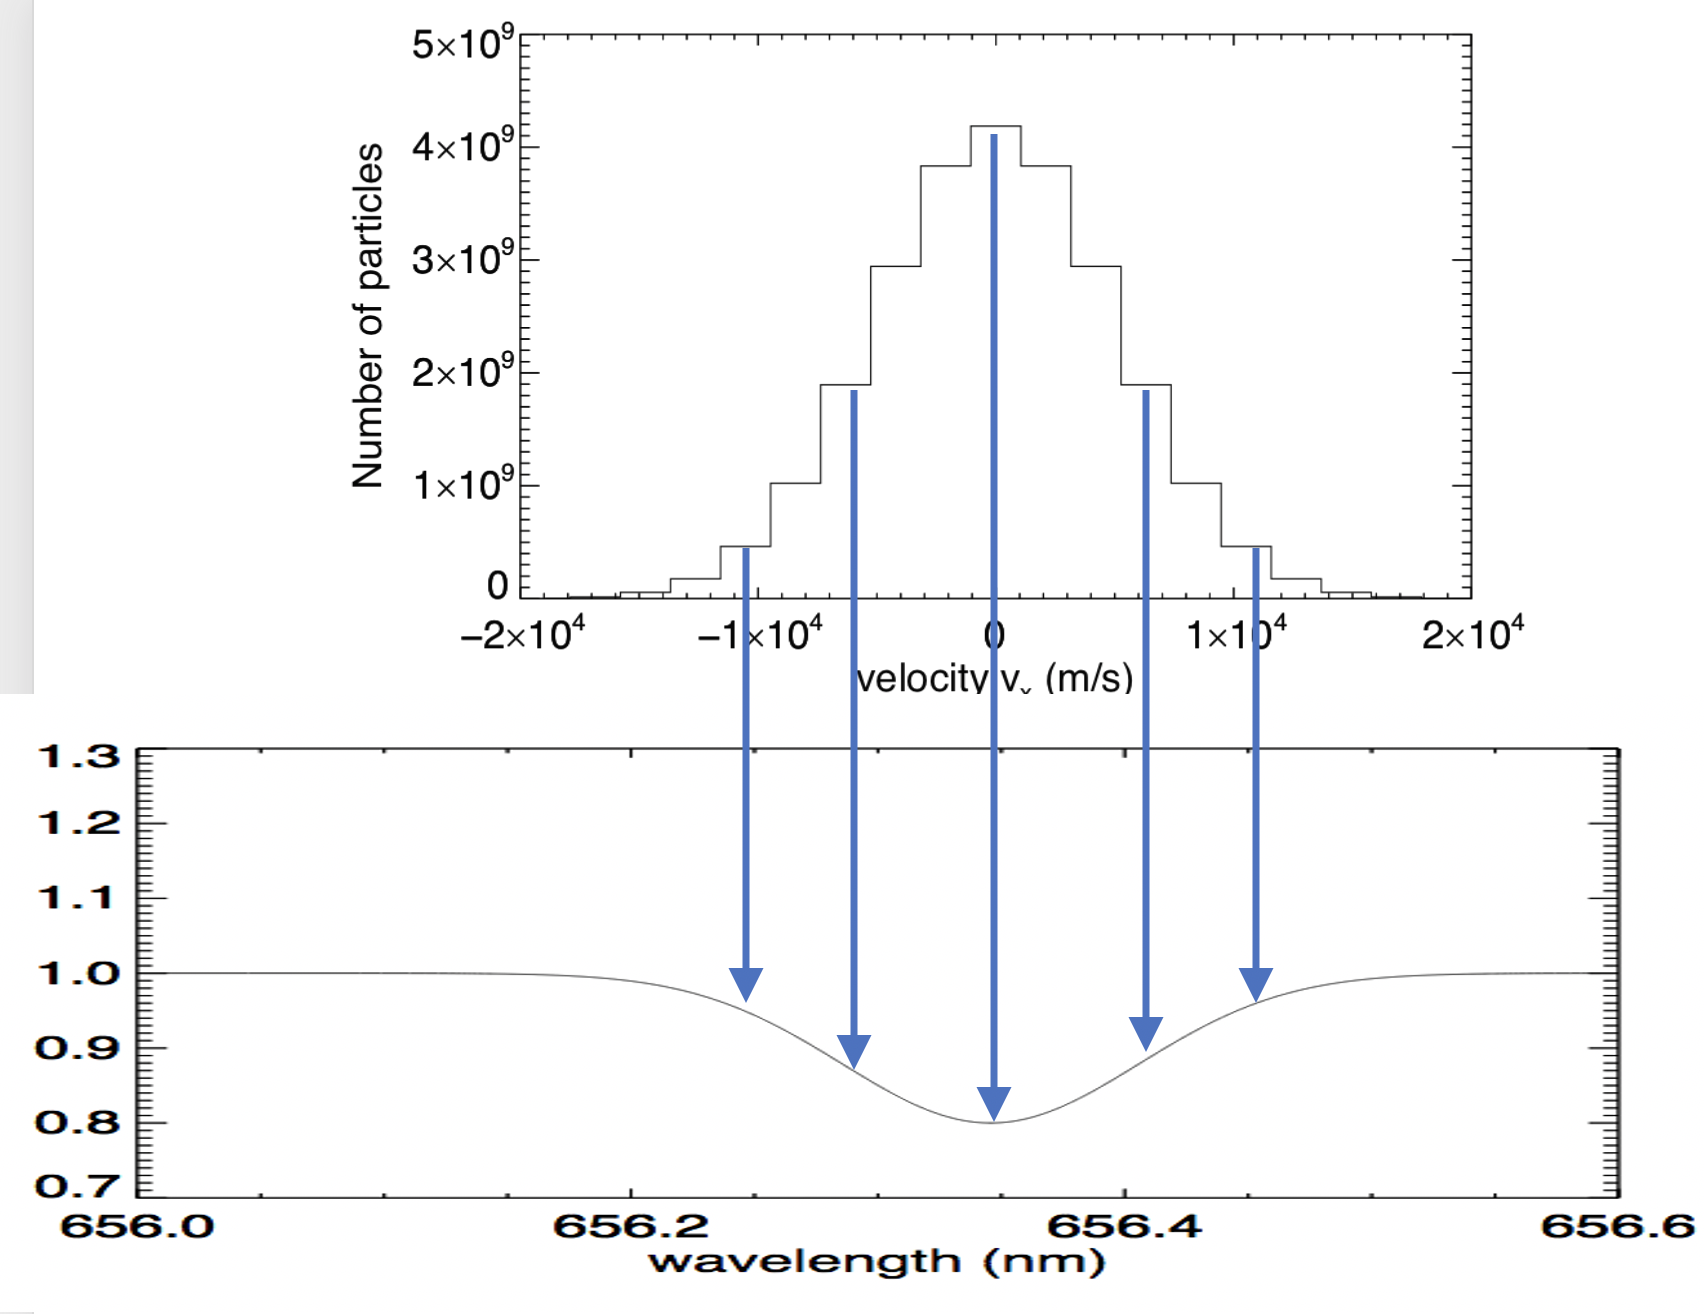
\includegraphics[scale=0.2]{media/linegen.png}}
{\small
Fordelingen av hastigheter er Gaussisk, altså er fordelingen av antall partikler som absorberer som funksjon av hastighet og dermed bølgelengde, Gaussisk. Dermed må også antall fotoner som blir absorbert og dermed fallet i fluksen også være Gaussisk. Toppen i Maxwell-Boltzmann er på 0 hastighet, dermed blir toppen eller bunnen i fluksen også på $\lambda_0$, dvs. ingen Doppler-effekt, slik som vi utledet for et par sider tilbake. Men hva med standardavviket $\sigma$? Tenk deg godt om og se om du kan se hva det må bli!
}
\hyperlink{linjeintro13b}{\pagebutton{Neste side}}
\end{frame}


\begin{frame}
\label{linjeintro13b}
\lastpagebutton{linjeintro13}
\centerline{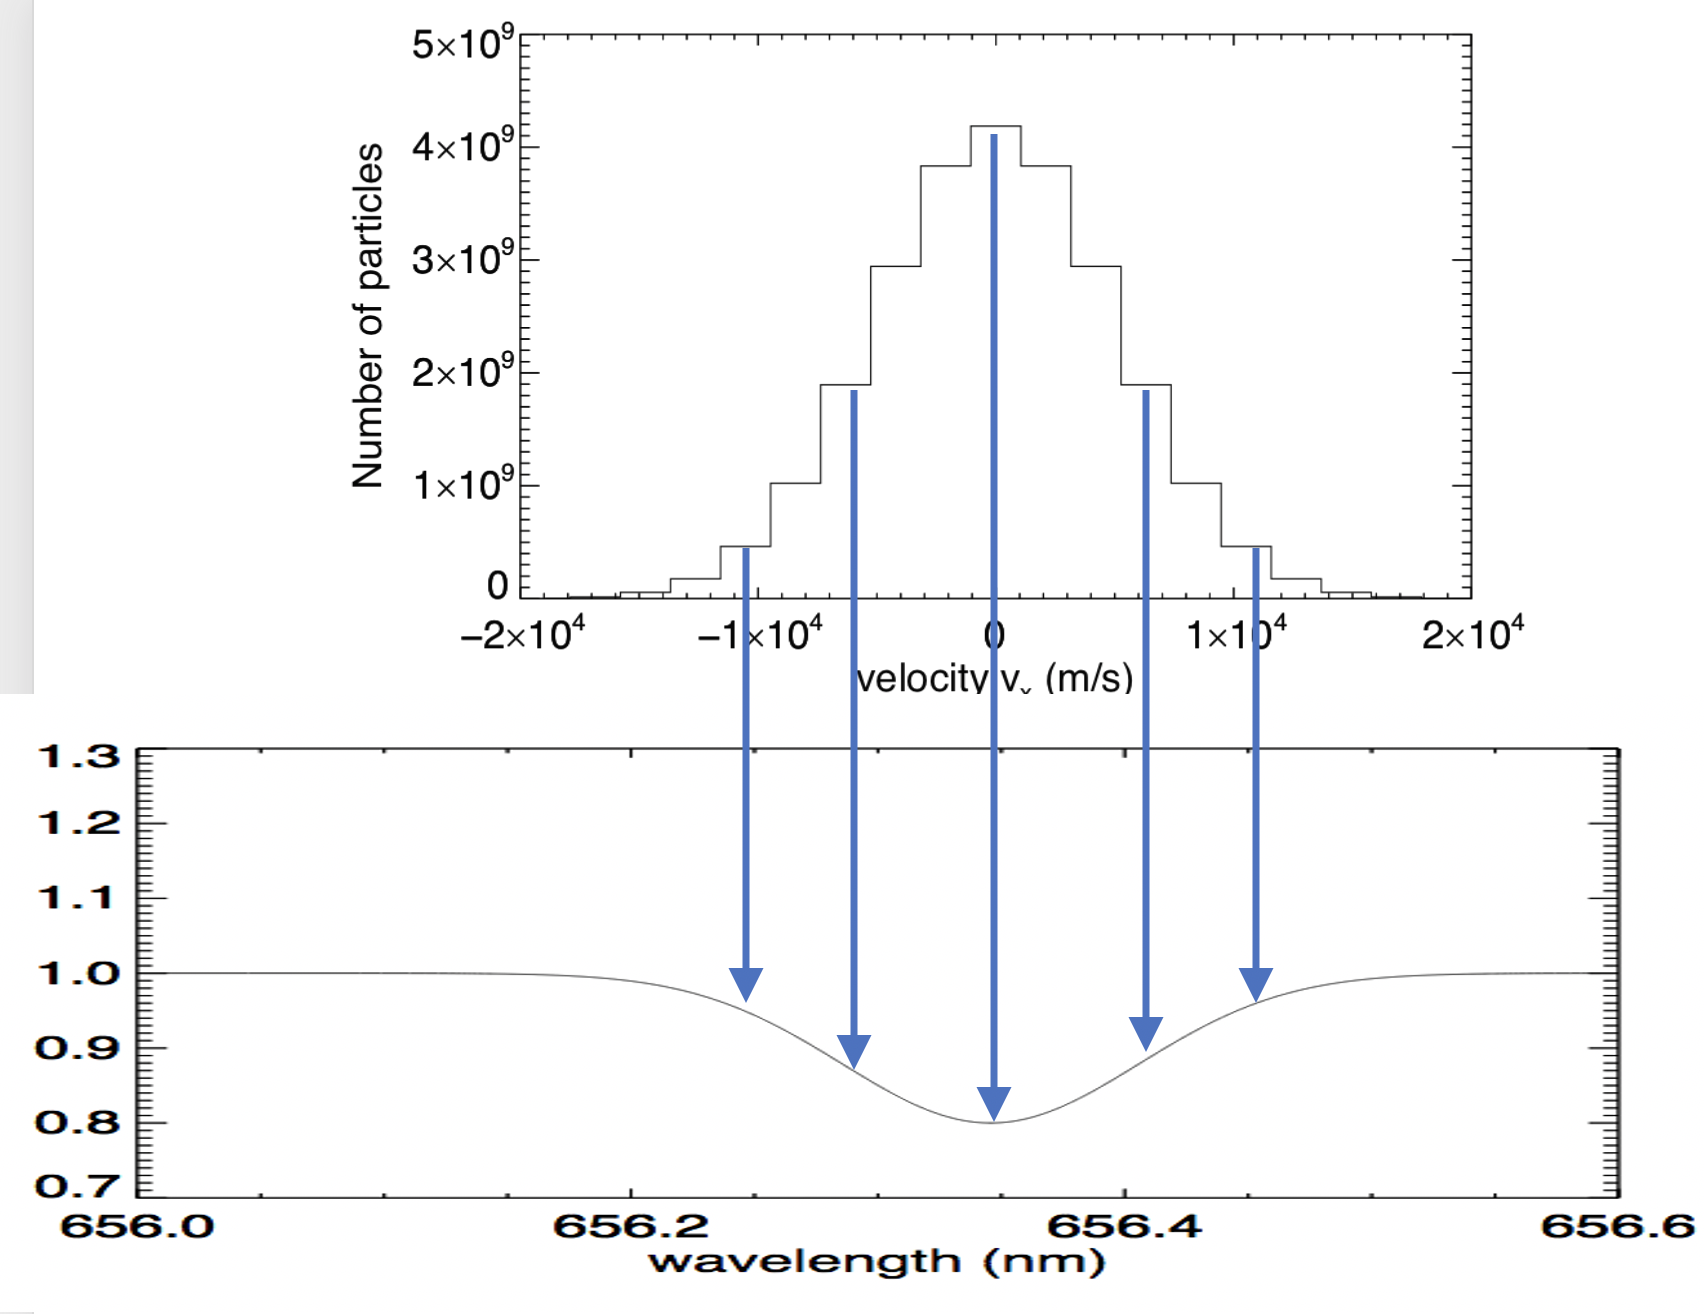
\includegraphics[scale=0.2]{media/linegen.png}}
Standardavvik for hastighet er $\sigma_v=\sqrt{\frac{kT}{m}}$. De partiklene som har $v_x$ lik dette standardavviket vil gi opphav til en Dopplereffekt $\Delta\lambda=\lambda_0\frac{v_x}{c}$ som insatt for $v_x$ gir $\Delta\lambda=\frac{\lambda_0}{c}\sqrt{\frac{kT}{m}}$ og som dermed tilsvarer standardavviket for spektrallinja og dermed også er et mål på bredden til linja. Dermed ser vi at vi fra bredden av spektrallinja har et direkte mål på temperaturen til gassen, gitt at du kjenner massen $m$ til atomene/molekylene.
\hyperlink{linjeintro14}{\pagebutton{Neste side}}
\end{frame}


\begin{frame}
\label{linjeintro14}
\lastpagebutton{linjeintro13b}
\centerline{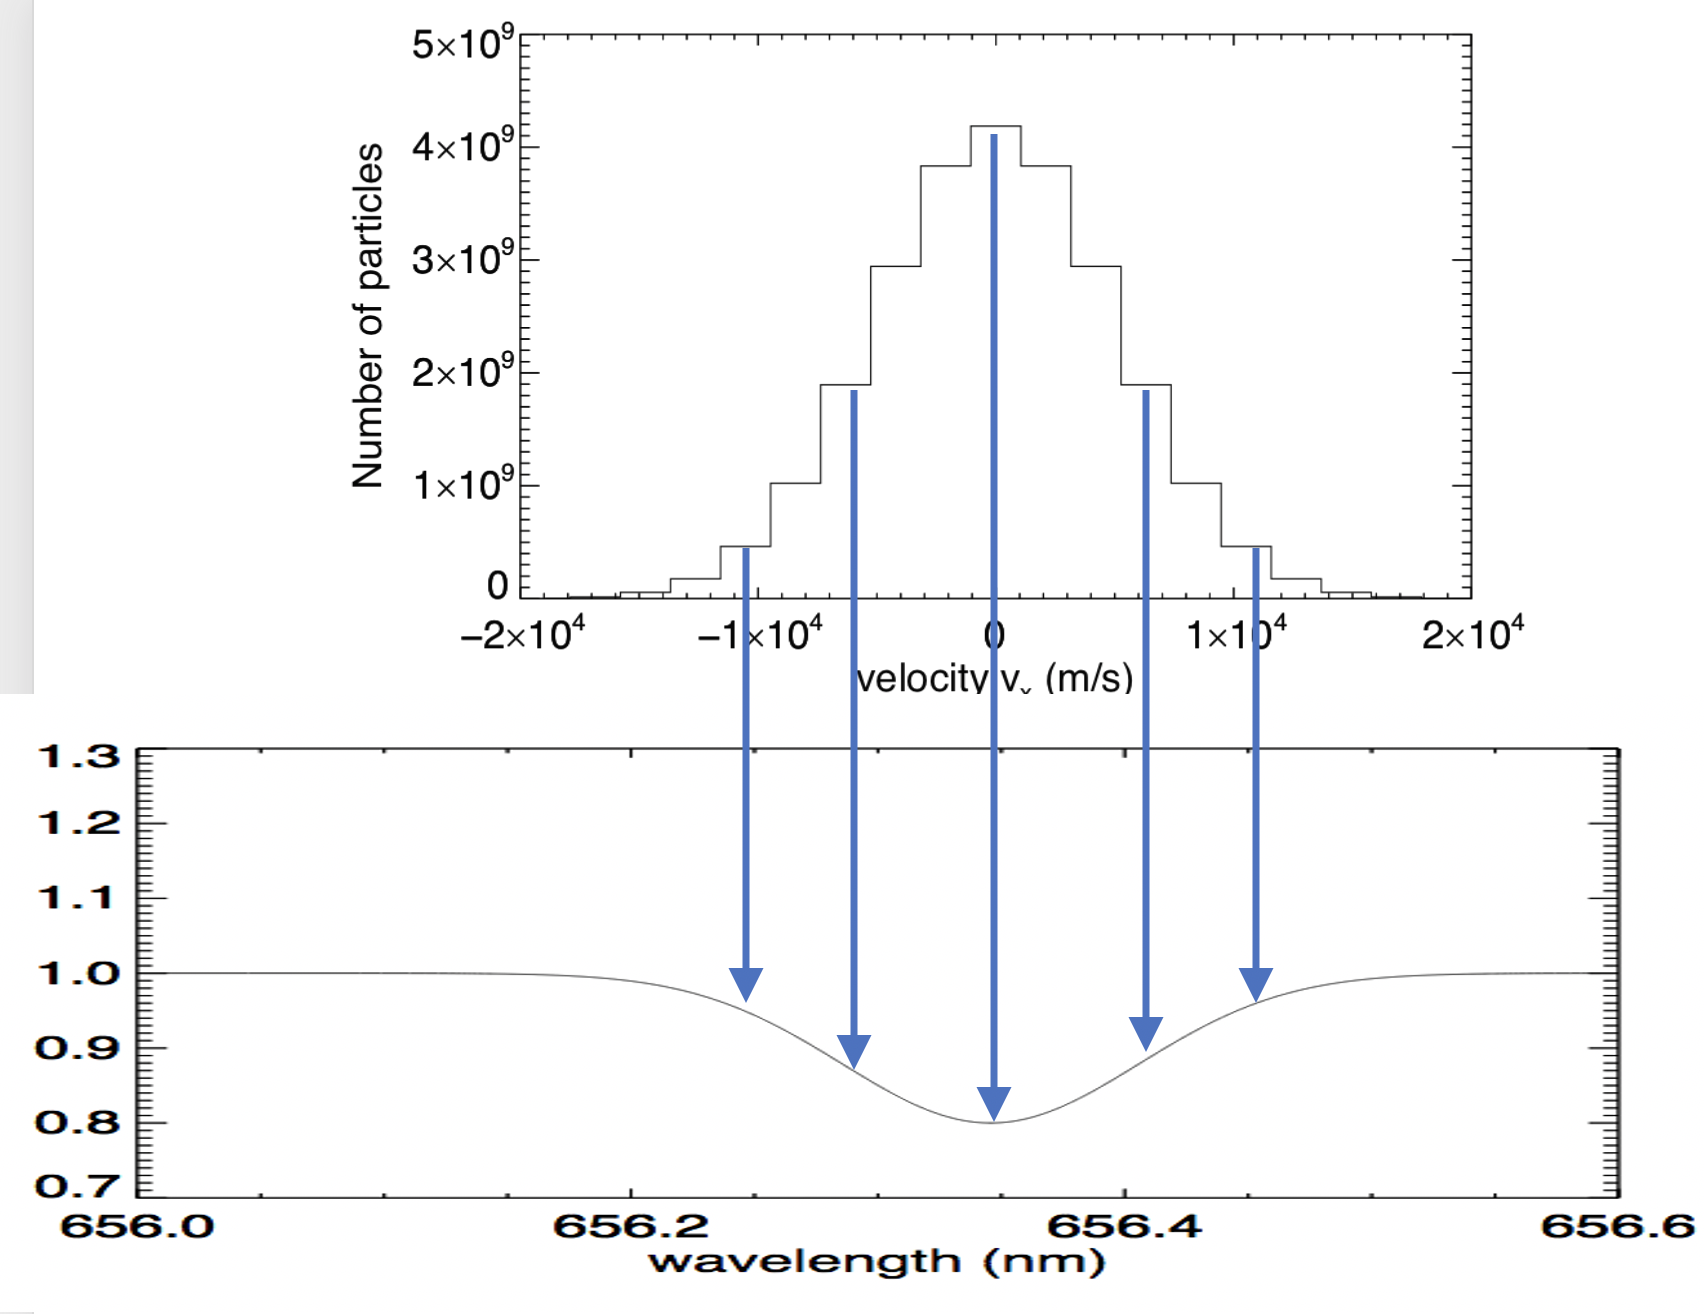
\includegraphics[scale=0.2]{media/linegen.png}}
{\small
Fluksen $F(\lambda)$ utenfor selve spektrallinja kaller vi kontinumsfluksen. Totalfluks i selve spektrallinja er altså kontimumsfluksen pluss formen på spektrallinja. Vi skal i det følgende anta at vi normaliserer fluksen $F(\lambda)$ slik at kontnumsfluksen er 1. Dermed blir $F(\lambda)=1$ utenfor spektrallinja, på begge sider. Minimumsfluksen (hvis vi antar absorpsjonslinje), kaller vi $F_\mathrm{min}$. Bølgelengden i sentrum kaller vi $\lambda_0$ og standardavviket $\sigma$. Kan du skrive et uttrykk for $F(\lambda)$ uttrykt kun ved $F_\mathrm{min}$, $\lambda_0$, $\sigma$ og selvfølgelig også $\lambda$? Tenk deg godt om og skriv ned et forslag før du blar om.
}
\hyperlink{linjeintro15}{\pagebutton{Neste side}}
\end{frame}

\begin{frame}
\label{linjeintro15}
\lastpagebutton{linjeintro14}
\centerline{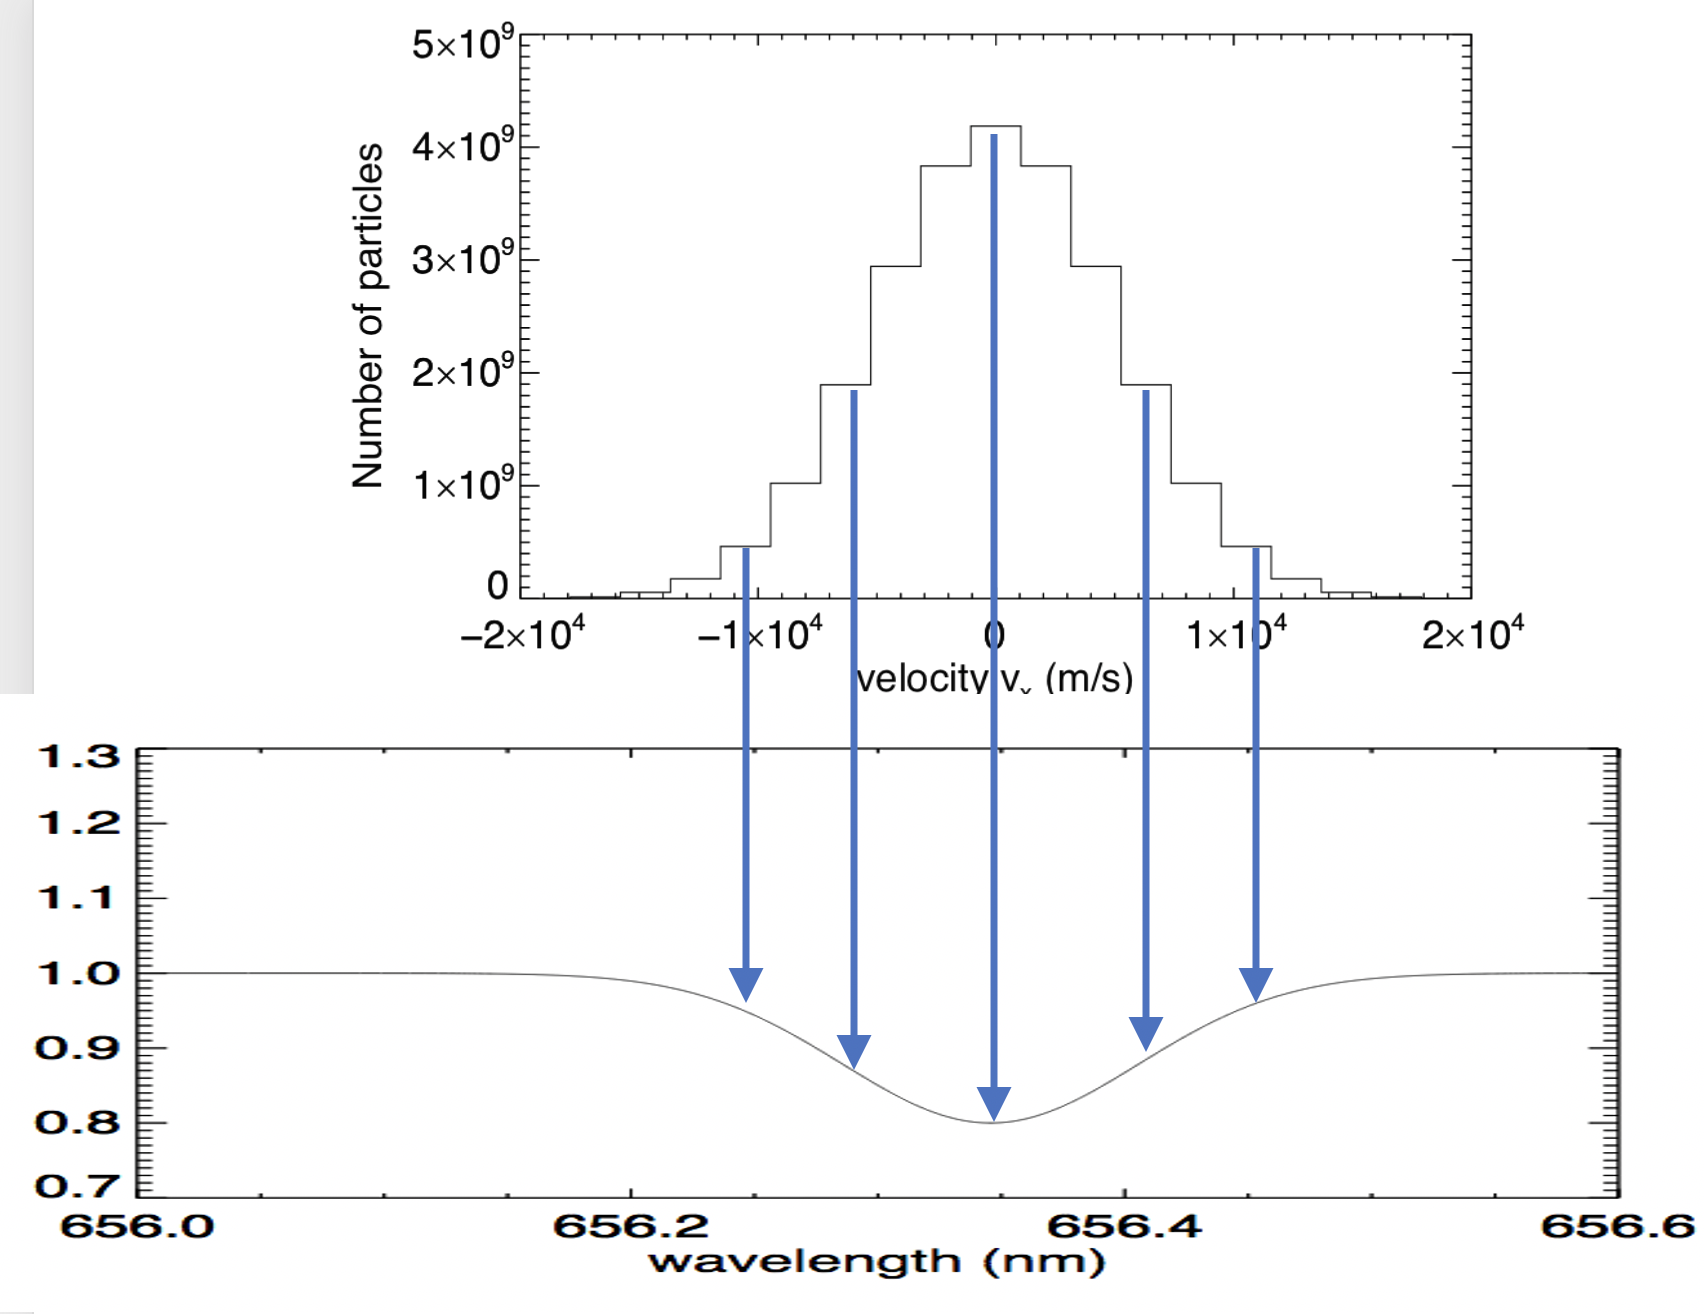
\includegraphics[scale=0.2]{media/linegen.png}}
Fikk du noe slikt?
\[
F(\lambda) = 1+(F_\mathrm{min}-1)e^{-\frac{(\lambda-\lambda_0)^2}{2\sigma^2}}
\]
Her ser vi at hvis eksponenten er 1 (altså $\lambda=\lambda_0$) så er $F(\lambda) = F_\mathrm{min}$, mens når vi er langt fra sentrum av linja og eksponenten dermed går mot 0 så får vi 1 (kontinumsfluksen). Og formen er Gaussisk med standardavvik $\sigma$. {\bf Hvis du ikke får dette til å stemme, kontakt foreleser/gruppelærer!}.
\hyperlink{pause}{\pagebutton{Neste side}}
\end{frame}



{
\setbeamercolor{background canvas}{bg=cyan}
\begin{frame}
\label{pause}
\hyperlink{linjeintro15}{\pagebutton{\small Forrige side}}
{\Huge
\centerline{Kaffe??? Er vel på tide...}
\centerline{
\includegraphics[scale=4]{media/drink-coffee.png}}\\
Kanskje en gåtur for å klarne tankene?
\vspace*{0.5cm}
Ihvertfall 10 min...
}\\
\vspace*{0.5cm}
\hyperlink{blue_nytema4}{\pagebutton{Har klarnet tankene nå!}}
\end{frame}
}



\renewcommand{\headline}{\small Observasjoner av spektrallinjer}
{
\setbeamercolor{background canvas}{bg=blue}
\begin{frame}
\label{blue_nytema4}
\hyperlink{linjeintro15}{\pagebutton{\small Forrige side}}
\nytemaside{storrelseklasser}
\hyperlink{linjeintro16}{\pagebutton{La oss nå se litt på observasjoner av disse linjene da!}}
\end{frame}
}


\begin{frame}
\label{linjeintro16}
\begin{columns}
\column{0.5\textwidth}
\lastpagebutton{linjeintro15}\label{obs}
{\small Og dermed er vi fremme ved den ene innleveringoppgaven 1D.6. Da får du et observert spektrum med støy:}
\centerline{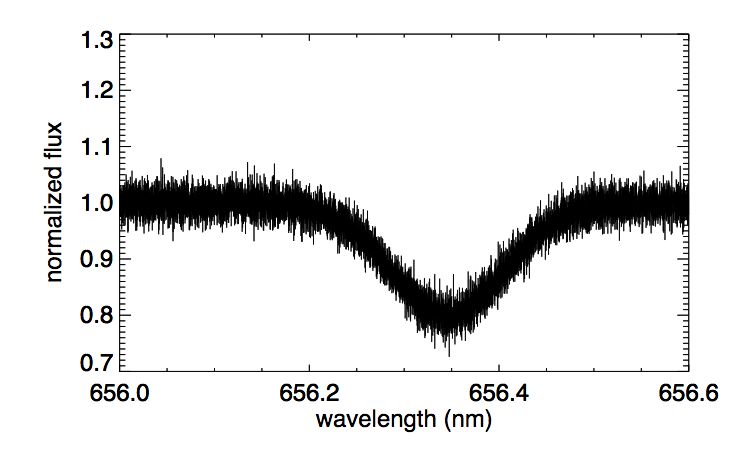
\includegraphics[scale=0.5]{media/noisyspectrum.png}}
{\small
Her skal du bruke minste kvadraters metode for å finne et estimat av den glatte underliggende kurven og dermed av temperaturen til gassen.
}
\column{0.5\textwidth}
{\small   Du kjenner nå modellen for $F(\lambda)$ og skal dermed tilpasse de ukjente parameterene $\lambda_0$, $\sigma$ og $F_\mathrm{min}$ på akkurat samme måte som i 1C. Egentlig kjenner du jo $\lambda_0$ som er senteret i spektrallinjen, men hvis stjerna har en hastighet i forhold til observatøren så får vi også en Dopplereffekt pga. egenhastigheten (peculiar velocity, se del 1C) og dermed endres senterlinja $\lambda_0$. Denne endringen i bølgelengde kan du bruke til å finne egenhastigheten til stjerna.
}
\hyperlink{linjeintro17}{\pagebutton{Neste side}}
\end{columns}
\end{frame}

\begin{frame}
\label{linjeintro17}
\lastpagebutton{linjeintro16}
{\bf Et lite tips på veien:} Når du skal finne intervaller for $\sigma$ ved avlesning så er det litt vanskelig da $\sigma$ ikke er en veldig intuitiv størrelse. Da er det mye lettere om du går veien via FWHM. Kikk tilbake på del 1A hvis du ikke husker hva FWHM var. Spesielt viktig her er sammenhengen mellom $\sigma$ og FWHM:
\[
\mathrm{FWHM}=2\sigma\sqrt{2\ln{2}}
\]

Bortsett fra det så er dette veldig likt det som du gjorde i 1C. Bruk tipsene der for å finne bugs i koden.\\
\textcolor{red}{Merk forbindelsen til del 1C i denne oppgaven: når du finner den forflyttede $\lambda_0$ så finner du hastigheten til stjerna på det gitte tidspunktet. Nå du så gjentar dette for observasjoner tatt på flere forskjellige tidspunkt så får du til slutt hastighetskurven til stjerna som du brukte i 1C til å finne ut om den har planeter og hvilke egenskaper disse planetene har.}
\hyperlink{linjeintro18}{\pagebutton{Neste side}}
\end{frame}



\begin{frame}
\label{linjeintro18}
\lastpagebutton{linjeintro17}
{\small I oppgave 1D7 som også er en innleveringsoppgave og som er spesielt viktig for prosjektstudentene, skal dere lete etter spektrallinjer i spektret til atomsfæren på planeten deres. Et spekter kan f.eks. se slik ut:}
\centerline{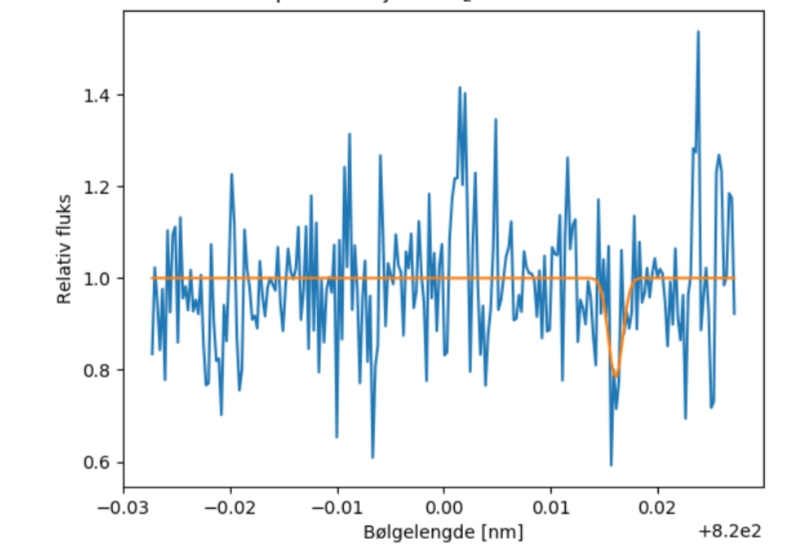
\includegraphics[scale=0.5]{media/noisy_chi2.png}}
{\small
I denne oppgaven vil standardavviket til støyen variere som funksjon av bølgelengde. Du skal dermed gjøre $\chi^2$ tilpasning istedenfor minste kvadrat (se igjen 1C for repetisjon!). I figuren ser du et eksempel på en tilpasset spektrallinje. {\bf Spørsmålet her blir hvordan du kan være sikker på om det faktisk er en spektrallinje her i det hele tatt?} 
}
\hyperlink{linjeintro19}{\pagebutton{Neste side}}
\end{frame}

\begin{frame}
\label{linjeintro19}
\lastpagebutton{linjeintro18}
\centerline{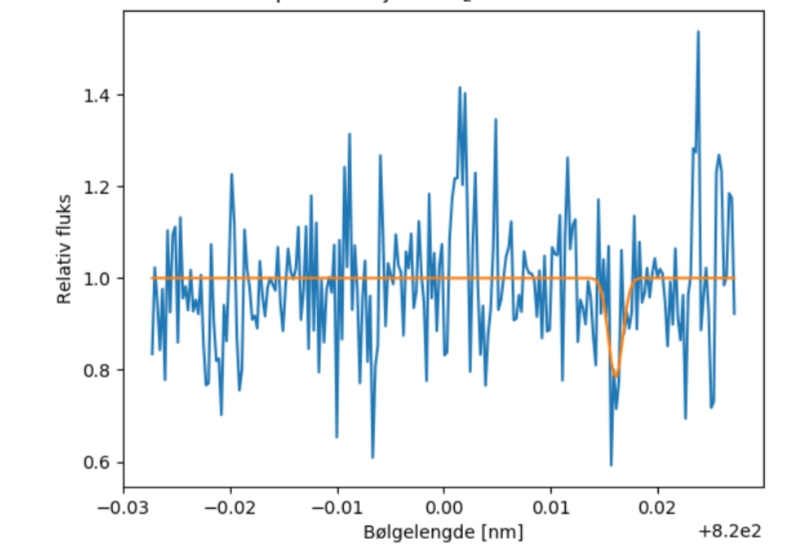
\includegraphics[scale=0.5]{media/noisy_chi2.png}}
{\small
Ser du at støyen har utslag som er like kraftige som spektrallinja som har blitt funnet. \textcolor{red}{Det er viktig å merke seg at minste kvadraters metode og $\chi^2$ metoden gjør en best mulig tilpasning selv om det i dette tilfellet godt kan være at det overhodet ikke er noen spektrallinje her! Da kan det være at den har prøvd å finne en Gaussisk grop inne i støy-fluktuasjonene!} Tenk gjennom hva du kan gjøre for å luke ut slike tilfeller (du vil aldri kunne luke disse ut med 100\% sikkerhet!). Hvilken strategi vil du bruke for å avgjøre om dette er en linje eller ikke?
}
\hyperlink{linjeintro20}{\pagebutton{Neste side}}
\end{frame}


\begin{frame}
\label{linjeintro20}
\lastpagebutton{linjeintro19}
\centerline{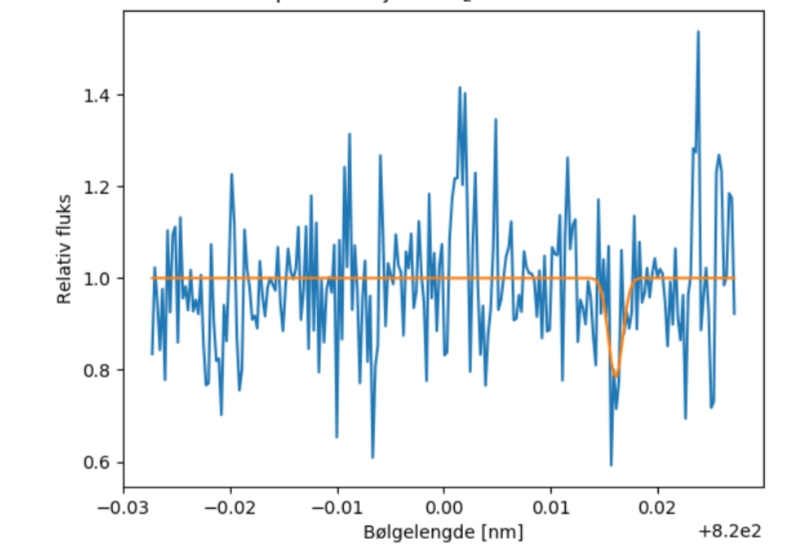
\includegraphics[scale=0.5]{media/noisy_chi2.png}}
{\bf Fler tips til dette vil du få i selve oppgaven og på gruppene hvis du er usikker.}
\hyperlink{blue_nytema5}{\pagebutton{Neste side}}
\end{frame}

\renewcommand{\headline}{\small Størrelseklasser}
{
\setbeamercolor{background canvas}{bg=blue}
\begin{frame}
\label{blue_nytema5}
\hyperlink{linjeintro20}{\pagebutton{\small Forrige side}}
\nytemaside{0}
\hyperlink{magnitudes1}{\pagebutton{Litt astronomi står på programmet...}}
\end{frame}
}

\begin{frame}
\label{magnitudes1}
\lastpagebutton{linjeintro20}\label{storrelseklasser}
Da har vi kommet til siste tema i del 1D. Dette dreier seg om en ny måleenhet for \textcolor{red}{fluks} og \textcolor{red}{luminositet} som brukes hyppig i astrofysikken og da spesielt blant de som gjør observasjoner med teleskop. {\bf Hvis du ikke har full kontroll på disse to begrepene, gå tilbake og repeter, evt. spør foreleser/gruppelærer} før du går videre!
\hyperlink{feil_magnitudes2}{\pagebutton{Neste side}}
\end{frame}

{
\setbeamercolor{background canvas}{bg=black}
\begin{frame}
\label{feil_magnitudes2}
\lastpagebutton{magnitudes1}
\centerline{\includegraphics[scale=0.2]{media/sky.png}}
\textcolor{white}{
{\tiny (bilde fra NASA/JPL)}\\
I bildet ser du massevis av objekter med forskjellig fluks. Noen objekter er veldig lysende med stor fluks, noen er svake og såvidt synlige og dermed med lav {\bf mottatt} fluks. Merk at vi her snakker om \textcolor{red}{mottatt} fluks, fluksen tatt ved observatøren. Fluksen rett ved objektet, den \textcolor{red}{utsendte} fluksen, er en helt annen. Dobbeltsjekk at du forstår dette og at du vet hvordan du kan regne fra utsendt fluks til motsatt fluks og tilbake igjen.
}
\hyperlink{feil_magnitudes3}{\pagebutton{Neste side}}
\end{frame}
}

{
\setbeamercolor{background canvas}{bg=black}
\begin{frame}
\label{feil_magnitudes3}
\lastpagebutton{feil_magnitudes2}
\centerline{\includegraphics[scale=0.2]{media/sky.png}}
\textcolor{white}{
{\tiny (bilde fra NASA/JPL)}\\
Den greske astronomen Hipparkhos (omkring 150 år før vår tidsregning) klassifiserte stjerner på nattehimmelen i 6 såkalte størrelseklasser (magnitudes). De aller sterkeste stjernene på himmelen var i størrelseklasse 1, mens de man såvidt kunne skimte med øyet var i størrelseklasse 6. Kan du tenke deg hva man idag bruker til å klassifisere stjernenes 'styrke' på himmelen?
}
\hyperlink{feil_magnitudes4}{\pagebutton{Neste side}}
\end{frame}
}


{
\setbeamercolor{background canvas}{bg=black}
\begin{frame}
\label{feil_magnitudes4}
\lastpagebutton{feil_magnitudes3}
\centerline{\includegraphics[scale=0.2]{media/sky.png}}
{\small

\textcolor{white}{
{\tiny (bilde fra NASA/JPL)}\\
Jepp, man bruker faktisk enda Hipparkhos sin skala, men man har gjort det litt mer vitenskapelig/matematisk. Hvor sterk vi ser en stjerne på himmelen er jo bare et mål på den mottatte fluksen. Hvis fluksen (lysenergi vi mottar per areal og tid) er stor, så ser stjerna sterk ut og motsatt. Øyet registrerer lysstyrke logaritmisk i fluks. Dermed har man definert det slik at et objekt som har 100 ganger større fluks en et annet objekt har en forskjell i størrelseklasse på 5. Dette stemmer ganske godt med Hipparkhos' opprinnelige klassifisering.
}
}
\hyperlink{feil_magnitudes5}{\pagebutton{Neste side}}
\end{frame}
}

{
\setbeamercolor{background canvas}{bg=black}
\begin{frame}
\label{feil_magnitudes5}
\lastpagebutton{feil_magnitudes4}
\centerline{\includegraphics[scale=0.2]{media/sky.png}}
{\small

\textcolor{white}{
{\tiny (bilde fra NASA/JPL)}\\
Så, da har vi det vi trenger. Anta at vi har to objekter, objekt 1 har fluks $F_1$ og størrelseklasser $m_1$. Tilsvarende har objekt 2 fluks $F_2$ og størrelseklasse $m_2$. Vi vet at hvis $F_2=F_2$ så er $m_1=m_2$. Vi har også definert at hvis $F_1=100F_2$ så er $m_2-m_1=5$ (\textbf{MERK: Størrelseklassen blir mindre når fluksen blir større, lav størrelseklasse betydde jo at stjerna var sterk!}.) Kan du finne en generell sammenheng mellom $F_1$, $F_2$, $m_1$ og $m_2$? Hint: her må det vel noe logaritmisk til (10-logaritme). Ikke gå videre før du har et forslag.
}
}
\hyperlink{feil_magnitudes6}{\pagebutton{Neste side}}
\end{frame}
}


{
\setbeamercolor{background canvas}{bg=black}
\begin{frame}
\label{feil_magnitudes6}
\lastpagebutton{feil_magnitudes5}
\centerline{\includegraphics[scale=0.2]{media/sky.png}}
{\small
\textcolor{white}{
{\tiny (bilde fra NASA/JPL)}\\
Hvis begge betingelser skal være oppfylt, hvilke av de følgende uttrykk kan det være? (det kan være flere enn et som er riktig). Merk at log=10-log!\\
\hyperlink{feilmag}{\choicebutton{\small$F_1=5\log{F_2}$}}\ \ \ \ \hyperlink{feilmag}{\choicebutton{\small$F_1=10^{(\log{F_2})/5}$}}\ \ \ \ \hyperlink{feilmag}{\choicebutton{\small$F_1-F_2=5\log{(m_1-m_2)}$}}\ \ \ \ \hyperlink{riktigmag}{\choicebutton{\small$F_1=F_{2}100^{(m_2-m_1)/5}$}}\ \ \ \ \hyperlink{feilmag}{\choicebutton{\small$F_1-F_2=10\log{((m_2-m_1)/5)}$}}\ \ \ \ \hyperlink{riktigmag}{\choicebutton{\small$m_1-m_2=-2.5\log{(F_1/F_2)}$}}\ \ \ \ \hyperlink{feilmag}{\choicebutton{\small$m_1=m_2\log{((F_1-F_2)/5)}$}}\ \ \ \ \hyperlink{feilmag}{\choicebutton{\small$m_1=m_{2} 10^{5(F_1-F_2)}$}}\ \ \ \ \hyperlink{feilmag}{\choicebutton{\small$m_1=m_{2} 5\log{(F_1-F_2)}$}}\ \ \ \ \hyperlink{feilmag}{\choicebutton{\small$m_1/m_2=100^{(5F_1/F_2)}$}}\ \ \ \ \hyperlink{feilmag}{\choicebutton{\small$F_1/F_2=100^{(5m_1/m_2)}$}}
}
}
\end{frame}
}


{
\setbeamercolor{background canvas}{bg=black}
\begin{frame}
 \label{feilmag}
\lastpagebutton{feil_magnitudes6}
\textcolor{white}{Har du sjekket skikkelig? Er det virkelig slik at når $m_1=m_2$ så blir $F_1=F_2$ for dette uttrykket? Er det også slik at når $F_1=100F_2$ så er $m_2-m_1=5$? Nei, begge er ikke oppfylt i dette uttrykket. Gå tilbake og sjekk igjen!}
\end{frame}
}

{
\setbeamercolor{background canvas}{bg=yellow}
\begin{frame}
\label{riktigmag}
\clastpagebutton{feil_magnitudes6}
Det er helt riktig! Ved å bruke at størrelseklassen er 5 ganger mindre hvis fluksen er 100 ganger større kan vi skrive at
\[
F_1=F_2 100^{(m_2-m_1)/5}
\]
Dette gir oss dermed
\begin{block}{\bf Sammenhengen mellom fluks og størrelseklasse (magnitude)}
\[
m_1-m_2=-2.5\log{(F_1/F_2)}
\]
der $m_1$ og $F_1$ er størrelseklassen og fluksen for objekt 1 mens $m_2$ og $F_2$ er størrelseklassen og fluksen for objekt 2.
\end{block}
Kan du se hvilke egenskaper ved objektet som avgjør hvilken størrelseklasse/fluks det har? Det er to egenskaper...
\hyperlink{red_magnitudes6b}{\pagebutton{Neste side}}
\end{frame}
}




{
\setbeamercolor{background canvas}{bg=red}
\begin{frame}
\label{red_magnitudes6b}
\lastpagebutton{riktigmag}
\textcolor{yellow}{
{\Large
Fant du virkelig to egenskaper???\\
Ikke gå videre før du har tenkt deg godt om!\\
}
}
\hyperlink{magnitudes7}{\pagebutton{Neste side}}
\end{frame}
}


\begin{frame}
\label{magnitudes7}
\lastpagebutton{red_magnitudes6b}
Nettopp ja! Fluksen avhenger jo av luminositeten og arealet som energien spres ut i! Men dette arealet avhenger jo av avstanden til objektet. Så luminositet og avstand alene avgjør fluksen og dermed størrelseklassen så lange vi antar at stråling ikke blir absorbert av f.eks. gass på veien til oss. Dermed ser vi at to stjerner med samme størrelseklasse kan ha veldig forskjellig luminositet hvis den ene er mye nærmere enn den andre. Størrelseklassen (og dermed hvor sterk stjerna/objektet ser ut til å være) sier oss altså ingenting om hvor sterkt dette objektet virkelig lyser (luminositeten).
\hyperlink{magnitudes8}{\pagebutton{Neste side}}
\end{frame}

\begin{frame}
\label{magnitudes8}
\lastpagebutton{magnitudes7}
Hvor sterkt objektet virkelig lyser måles jo med luminositet, men vi har et størrelseklassemål for dette også.
\begin{block}{Tilsynelatende og absolutt størrelseklasse (appaerent and absolute magnitude)}
Den størrelseklassen vi har snakket om så langt er et mål på fluksen vi mottar fra objektet, og avhenger dermed av luminositeten og avstanden til objektet. Dette kaller vi {\bf tilsynelatende størrelseklasse} og vi bruker den matematiske betegnelsen $m$. Vi kan også definere {\bf absolutt størrelseklasse} som kun avhenger av luminositeten til objektet og betegnes matematisk med $M$. {\it Absolutt størrelseklasse er den tilsynelatende størrelseklassen objektet ville hatt dersom vi hadde flyttet objektet til en avstand av 10pc}
\end{block}
\hyperlink{magnitudes9}{\pagebutton{Neste side}}
\end{frame}

\begin{frame}
\label{magnitudes9}
\lastpagebutton{magnitudes8}
Dersom vi flytter alle objekter i universet til en avstand av 10pc, så vil den tilsynelatende lysstyrken vi ser på himmelen være et mål på hvor sterkt objektet faktisk lyser, siden avstanden nå er den samme for alle objekter. \textcolor{red}{Dermed er absolutt magnitude et annet mål på luminositeten.} La oss prøve å finne en sammenheng mellom den tilsynelatende størrelseklassen $m$ og den absolutte størrelseklassen $M$ til et objekt. {\bf Kan du tenkte deg hvilken egenskap ved objektet denne sammenhengen må avhenge av?}
\hyperlink{magnitudes10}{\pagebutton{Neste side}}
\end{frame}


\begin{frame}
\label{magnitudes10}
\lastpagebutton{magnitudes9}
Ganske riktig, på samme måte som at {\bf sammenhengen mellom mottatt fluks og luminositet avhenger av avstanden}, så må det {\bf samme gjelde for tilsynelatende og absolutt størrelseklasse.} Du skal nå prøve å selv komme frem til sammenhengen mellom $m$ og $M$:
\begin{itemize}
\item Anta at du har et objekt, vi kaller det objekt 1, med tilsynelatende størrelseklasse $m_1$, i avstand $r$. 
\item Så har du et helt identisk objekt i en avstand av 10 pc, som du observerer med tilsynelatende størrelseklasse $m_2$. Denne tilsynelatende størrelseklassen tilsvarer jo da også den absolutte størrelseklassen $M$ for begge objekter siden objektene er identiske og det siste objektet befinner seg i en avstand av 10 pc. 
\item Før du blar om, bruk sammenhenger du kjenner mellom fluks og luminositet samt definisjonen av tilsynelatende størrelseklasse til å finne sammenhengen mellom $m$ og $M$.
\end{itemize}
\hyperlink{magnitudes11}{\pagebutton{Neste side}}
\end{frame}


\begin{frame}
\label{magnitudes11}
\lastpagebutton{magnitudes10}
Kom du frem til at
\begin{block}{sammenhengen mellom tilsynelatende og absolutt størrelseklasse er}
\[
m-M=5\log(\frac{r}{10pc})
\]
\end{block}
???\\
Hvis ikke, ta en kikk på \href{https://www.uio.no/studier/emner/matnat/astro/AST2000/h20/undervisningsressurser/interaktive-forelesningsnotater/1d/videoer/video1d_6.mp4}{denne videoen}\\
\hyperlink{magnitudes11b}{\pagebutton{Neste side}}
\end{frame}


\begin{frame}
\label{magnitudes11b}
\lastpagebutton{magnitudes11}
Hvis vi tar en kikk på uttrykket for tilsynelatende størrelseklasse en gang til:
\[
m_1-m_2=-2.5\log{(F_1/F_2)}
\]
så ser vi at du trenger en annet objekt 2 med kjent fluks og størrelseklasse for å kunne finne størrelseklassen til objekt 1! Vi trenger å {\it kalibrere} størrelseklasseskalaen. I mange år har stjerna Vega blitt brukt til dette, denne definerte man til å ha tilsynelatende størrelseklasse 0 (i dag brukes en noe annen definisjon, men det skal vi ikke snakke nærmere om her). Merk at Hipparkhos sin skala gikk fra 1 til 6 der 1 var de sterkeste stjernene på himmelen. Med den matematiske definisjonen så kan vi altså gå under 1 og over 6. En stjerne med størrelseklasse 6 også med den matematiske definisjonen en stjerne som såvidt er synlig med øyet, men med teleskop kan vi i dag se svake objekter med størrelseklasse langt større enn 6. 
\hyperlink{magnitudes12}{\pagebutton{Neste side}}
\end{frame}

\begin{frame}
\label{magnitudes12}
\lastpagebutton{magnitudes11b}
Himmelens sterkeste stjerne, Sirius, har negativ tilsynelatende størrelseklasse på -1.46. Sola har tilsynelatende størrelseklasse på -26.74. I andre enden av skalaen så kan romteleskopet Hubble observere objekter så svake at de har tilsynelatende størrelseklasse større enn 30. For størrelseklassen til flere objekter, se \href{https://en.wikipedia.org/wiki/Apparent\_magnitude}{ tabellen i bunnen av denne Wikipedia-artikkelen}.
\hyperlink{oppsummering}{\pagebutton{Neste side}}
\end{frame}

\begin{frame}
\label{oppsummering}
\hyperlink{magnitudes12}{\pagebutton{\small Forrige side}}\href{https://nettskjema.no/a/160193}{\Changey[1][yellow]{2} \Changey[1][yellow]{-2}}
Gratulerer, del 1D er overstått. Du bør nå:
\begin{itemize}
\item kjenne til hvilke kilder til informasjon vi har om universet,
\item kunne de viktigste prosessene som genererer elektromagnetisk stråling i verdensrommet,
\item vite hva en romvinkel er,
\item kunne forstå, definere og regne med uttrykkene fluks, luminositet, intensitet samt fluks og luminositet per bølgelengde,
\item vite hva et sort legeme er og egenskapene til strålingen det sender ut,
\item forstå hvordan en spektrallinje (emisjon og absorpsjon) dannes, hvilken form den har, hva som avgjør dens form og dens bredde,
\item estimere en tilpasning til en spektrallinje fra data med støy,
\item kunne definere og regne med visuelle og absolutte størrelseklasser.
\end{itemize}
\textcolor{red}{Flott hvis du nå kan klikke på smilefjesene over og fortelle hva du synes om dette interaktive forelesningsnotatet. Hva var bra og nøyaktig hva kan forbedres? All ris og ros mottaes med takk!}
{\bf Det anbefales nå at du sjekker \href{https://www.uio.no/studier/emner/matnat/astro/AST2000/h21/undervisningsmateriell/kortsvarsoppgaver/del1d.pdf}{kortsvarsoppgavene} til del 1D for å kontrollere at du har forstått stoffet. Kan du svare på disse, blir det lettere å bruke kunnskapen din i oppgavene/prosjektet. Noen av disse kommer på eksamen.}\\
\end{frame}



\end{document}

